\chapter{Results from Lennard-Jones simulations \label{ch:ParticleModelsResults}}
Here we report the outcome of computer simulations of deformation of Lennard-Jones systems, using the system and the techniques described in \autoref{ch:ParticleModels}. The general idea is simple: after samples are prepared, they are subjected to a series of oscillatory athermal deformation cycles. Our simulations thus extend those performed in \cite{lacks2004energy}, where samples were subjected to a single deformation semicycle. As a consequence of oscillatory deformation, particles in the system do rearrange, so that their positions and quantities as the average energy change as more and more oscillations are performed. In this chapter, we show that the way in which a system evolves depends crucially on the amplitude of oscillation $\gamma_{max}$, showing a phenomenology similar to that observed experimentally in dilute noncolloidal suspensions under oscillatory shear \cite{corte2008random}.  
The main findings presented here have been published in \cite{fiocco2013oscillatory}.

\section{Kob-Andersen Lennard-Jones mixtures (KA)}
In the simulations presented in this chapter, we consider systems of particles interacting via the LJ potential in \autoref{eq:BinaryLennardJonesPotential}, of sizes equal to $N=500, 4000, 32000$. The composition and pair potential parameters $\epsilon_{\alpha \beta}$ and $\sigma_{\alpha \beta}$ are those of introduced by Kob and Andersen (KA) in \cite{kob1994scaling} and are listed in \autoref{tab:KAParameters}.
This system has been chosen because it's one of the most popular choices in the literature to study the dynamics of dense viscous liquids \cite{binder2011glassy}. This in turn is due to the simplicity of the potential and the resistance to crystallization \cite{toxvaerd2009stability} that the model has.
\begin{table}
\centering
\begin{tabular}{ccc}
\toprule
$\alpha \beta$	&	$\epsilon_{\alpha \beta}$	&	$\sigma_{\alpha \beta}$	\\ 
\midrule
AA		&	1				&	1	 			\\
AB		&	1.5				&	0.8	 			\\
BB		&	0.5				&	0.88	 		\\
\bottomrule 
\end{tabular}
\caption{Values of the parameters of the Kob-Andersen (KA) binary Lennard-Jones mixture. Additional parameters are the overall number density $\rho = 1.2$ and the relative concentrations $c_{A} = 0.8$ and $c_{B} = 1 - c_{A} = 0.2$.}
\label{tab:KAParameters}
\end{table}

The system is simulated using LAMMPS (Large-scale Atomic/Molecular Massively Parallel Simulator) \cite{plimpton1995fast}. The choice of LAMMPS as the code to run the LJ simulations has been made for several reasons: it is able to perform molecular dynamics in different ensembles (and more specifically at constant $N, V, E$ and $N, V, T$) and potential energy minimization using different minimization strategies; it is fast\footnote{One of the very early stages of this thesis work consisted in writing a Fortran code able to perform molecular dynamics for a single component LJ system in the canonical ensemble using the Nos\'e-Poincar\'e \cite{nose2001improved} integrator, using \emph{cell lists} \cite{frenkel2001understanding}. On the same tasks and running on a single CPU, LAMMPS was on average at least 5 times faster.}, designed to run efficiently in parallel on multiple CPUs to handle large systems. Its source code is open, freely available, thoroughly documented and supported by a large community. Incidentally, LAMMPS allows the same simulation scripts to be run on both CPU and GPU architectures with very little modifications. \\
A cut-off is used to truncate the interaction and thus speed up the molecular dynamics (as described in \autoref{sec:MolecularDynamics}), and this is chosen to be set at $2.5 \sigma_{\alpha \beta}$ for the different species. The potential is cut and shifted, as in \cite{lacks2004energy}, to make a direct comparison of the results easier. The modified form of the potential thus reads
\begin{equation}
	\phi^{\mathrm cut-shift}_{\alpha \beta}(r) = 
	\left\{ 
	\begin{array}{rl}
		4\epsilon_{\alpha \beta} \left[ \left( \frac{\sigma_{\alpha \beta}}{r} \right)^{12} - \left( \frac{\sigma_{\alpha \beta}}{r} \right)^{6} \right] + c_{\alpha \beta} & \text{if } r < 2.5 \sigma_{\alpha \beta}  \\
		0 & \text{if } r \geq 2.5 \sigma_{\alpha \beta}
	\end{array}
	\right.
	\label{eq:BinaryLennardJonesPotentialCutAndShifted}
\end{equation}

and $c_{\alpha \beta}$ has the value such that $\phi^{\mathrm cut-shift}_{\alpha \beta}(2.5 \sigma_{\alpha \beta}) = 0$, and the pair potential is thus continuous at $r = 2.5 \sigma_{\alpha \beta}$. From the energy landscape point of view, \autoref{eq:BinaryLennardJonesPotentialCutAndShifted} implies that the landscape is continuous, and has no abrupt ``cliffs'' or steps.

\section{Preparation of the samples - equilibrium simulations}

Before starting an AQS deformation, initial inherent configurations need to be generated. To do so, we create configurations equilibrated at some temperature $T$ using the Nos\'e-Hoover thermostat and bring them to the inherent structure of the basin they belong to using the conjugate-gradient (CG) algorithm. In this thesis we use the implementation of the Polak-Ribi\`ere version of the CG algorithm\footnote{A pedagogical introduction to the CG method is given in \cite{shewchuk1994introduction}, whereas a useful comparison between different minimization strategies in order to find inherent structures is given in \cite{chakravarty2005generating}.} coded in LAMMPS \cite{plimpton1995fast}.
To equilibrate configurations, particles are initially placed at random in a simulation box. The consequence of this is that some of their centers can be very close to each other, and in that case will strongly repel each other (the force originating from \autoref{eq:BinaryLennardJonesPotential} at small $r$ is strongly repulsive). An energy minimization is thus applied to obtain a relaxed configuration\footnote{In principle, one could think of starting a simulation from an unrelaxed configuration and thermostating it at some $T$ using the Nos\'e-Hoover thermostat or similar schemes, but this would not be very practical due to the large initial forces that generate from particle overlaps. Because of such forces, the simulation would need very small integration times not to lose numerical stability.} characterized by less intense pair forces. 
Then, a set of velocities extracted from the Maxwell distribution at a given $T$ is assigned to the particles, and the trajectories of the particles are integrated numerically using the Nos\'e-Hoover scheme implemented in LAMMPS.
After an initial transient of duration $\tau_{t}$, the simulation is expected to start following an equilibrium trajectory so that the system visits configurations $\mathbf{R_{i}}$ with a probability density proportional to the Boltzmann factor $\exp(-\beta U(\mathbf{R_{i}}))$. 
Only once that equilibrium has been reached configurations can be recorded and used to calculate thermodynamical averages appropriate to the temperature $T$ \cite{frenkel2001understanding}. It is thus important to have a reliable estimate of $\tau_{t}$, in order to discard from the analyses configurations sampled during the initial transient out of equilibrium.
To do so, the potential energy $U$ is fit to the form $U(t) = (U(0) - U_{eq}) e^{-t/\tau_{t}} + U_{eq}$, and only configurations sampled for $t < \tau_{t}$ are considered for further analysis.
To have a more precise estimate of $\tau_{t}$, these configurations can be used to measure a \emph{decorrelation time} $\tau_{r}$ needed to the system to reach a state that has no relation with its initial one\footnote{This $\tau_{r}$, intuitively, is the time needed to the system to move in configuration space to a state which is as far (on average) as a state picked at random with a probability $\exp(-\beta U(\mathbf{R}))$.}.
Our measure of correlation of choice is the self part of the intermediate scattering function\footnote{Another choice for $\tau_{t}$ and $\tau_{r}$ could have been the correlation time of $U$ \cite{statfor, allen1989computer}.} \cite{hansen1990theory, schroder2000crossover}. 
Given a trajectory $\mathbf{R}(t)$ such that particles are located at $\mathbf{r_{1}}(t), \mathbf{\ldots}, \mathbf{r_{N}}(t)$, the self intermediate scattering function is defined as
\begin{equation}
	F_{s}(\mathbf{k}, t) = \frac{1}{N} \langle \sum_{i=1}^{N} \exp(-i \mathbf{k} \cdot (\mathbf{r_{i}}(t_{0} + t) - \mathbf{r_{i}}(t_{0}))) \rangle 
	\label{eq:IntermediateScattering}
\end{equation}
It follows from the definition that if the particles don't move from $t_{0}$ to $t_{0} + t$, then $F_{s} = 1$, because all the values in the exponential in \autoref{eq:IntermediateScattering} are equal to zero. If particles move, the real part of $F_{s}$ will have a lower value. One can calculate \autoref{eq:IntermediateScattering}  by summing over the positions of the $A$ particles only, thus obtaining $F_{sA}$.
We define $\tau_{r}$ as the time needed to the real part of $F_{sA}(k, t)$ to decay to 0.1, and we make the further assumption\footnote{In other words, we assume that the time needed to reach equilibrium from the initial non-equilibrium state is comparable to that needed to the system to reach independent states once in equilibrium.} that $\tau_{t} = \tau_{r}$.
Incidentally, the value of $\tau_{r}$ strongly depends on $T$. Intuitively, this is because at low temperatures the system moves slower in configuration space and is also more prone to be trapped in a valley of the potential energy landscape, with high potential energy barriers around it that prevent it from exploring the configuration space. More specifically, the binary KA is known to exhibit a dependence of $\tau_{r}$ on $T$, as shown in \autoref{fig:IntermediateScatteringKA}. This is a typical feature of glasses, that show a dramatic slowing down of their dynamics as the temperature is lowered below some $T_{g}$. This can be seen in more intuitive terms in \autoref{fig:MSDKA}, where the mean squared displacement of our KA system is plotted as a function of temperature. Clearly, as temperature is lowered, the system takes more and more time to move away from its initial configuration at $t=t_{0}$.

\begin{figure}[!h] 
\centering 
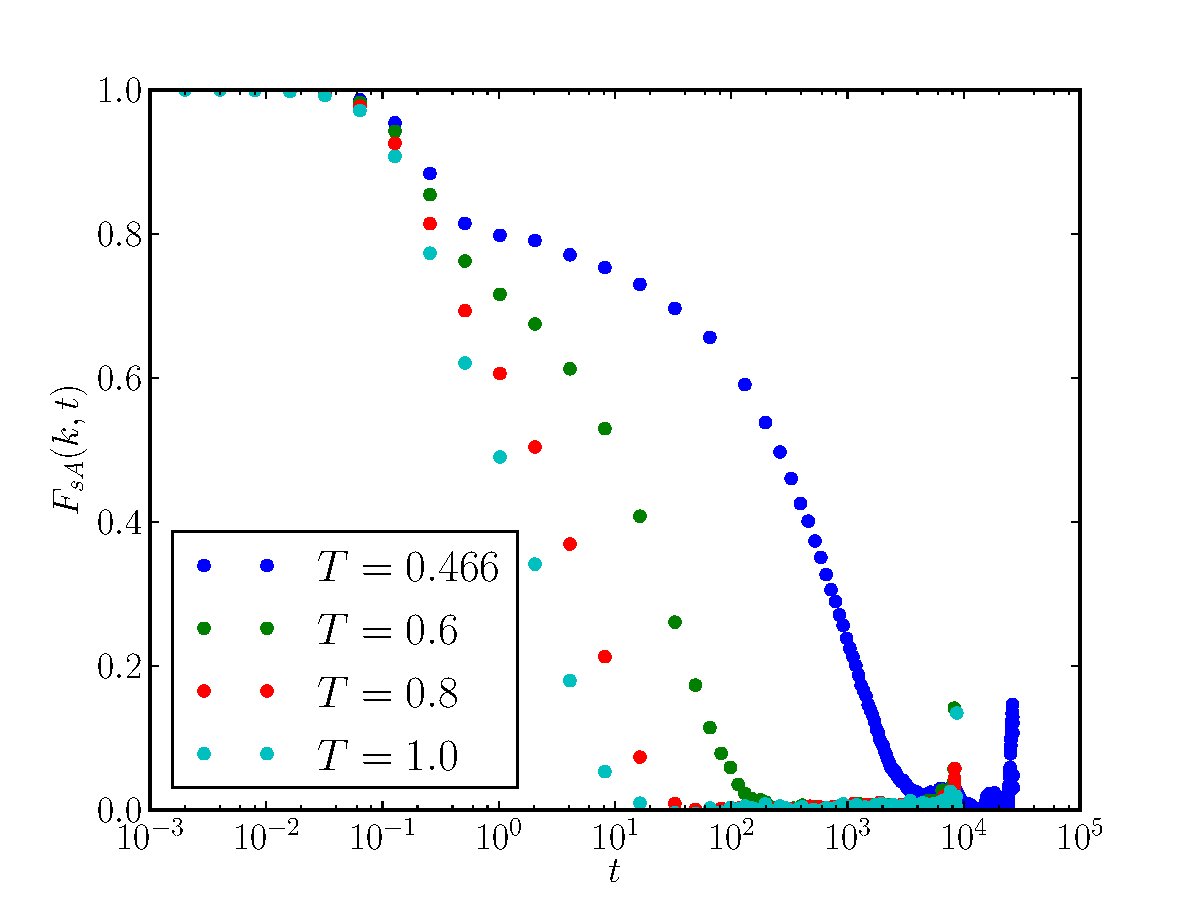
\includegraphics[width=0.8\textwidth]{IntermediateScatteringKA500.pdf} 
\caption{Self intermediate scattering function $F_{sA}(k,t)$ as a function of time obtained from KA samples with $N=500$ and equilibrated at different temperatures, at $k = 7.251$. At high $T$ the decay is exponential. At low $T$ the decay is slower, and has a more complicated two-step decay form. \label{fig:IntermediateScatteringKA}}
\end{figure}

\begin{figure}[!h] 
\centering 
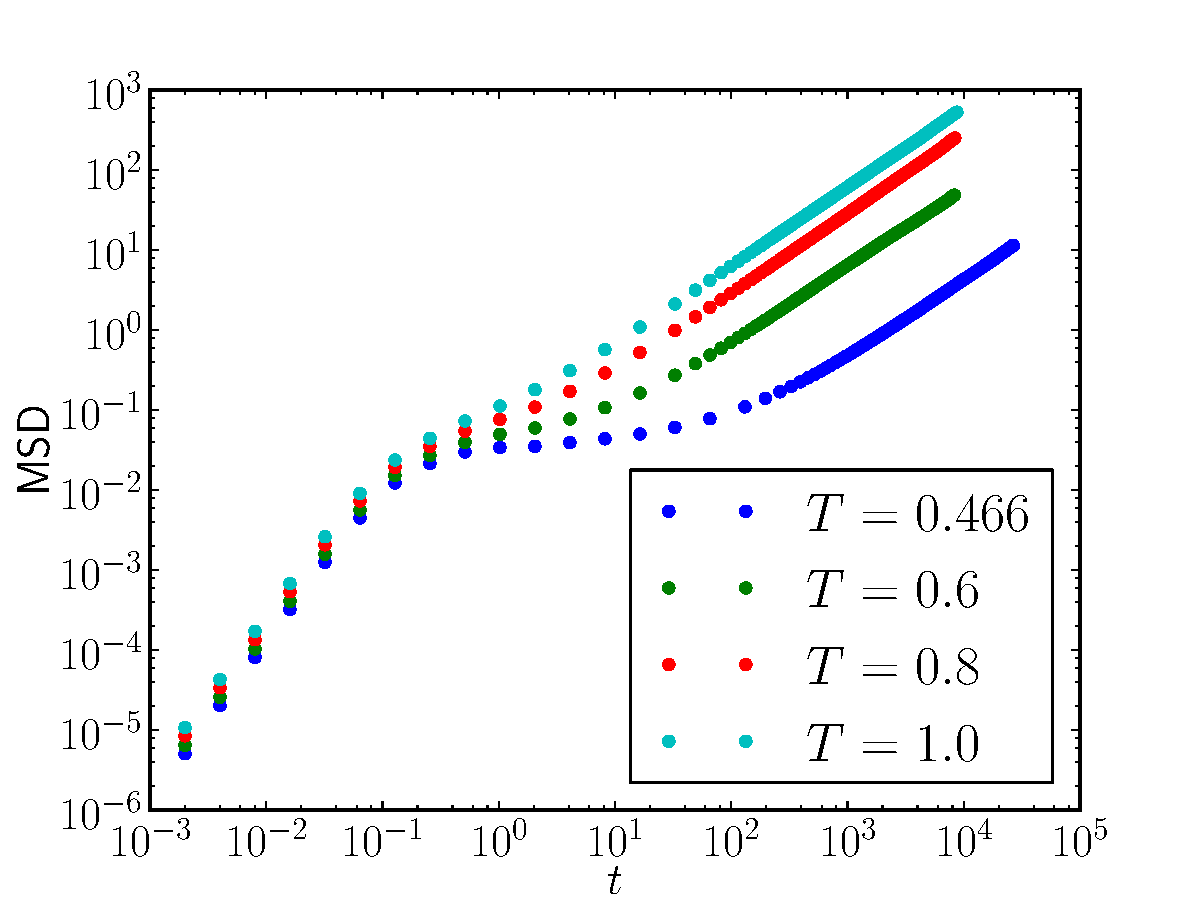
\includegraphics[width=0.8\textwidth]{MSDKA500.pdf} 
\caption{Mean squared displacement for the same systems described in \autoref{fig:IntermediateScatteringKA}. For all $T$ at short times the systems are ballistic, and the MSD has a quadratic dependence on time. At larger times the systems become all diffusive, as the MSD is linear in time. This happens only at large times for low $T$. At low $T$, particles spend a long time in the neighborhood of the $t = 0$ configuration before they start diffusing away from it. For this reason, the diffusion constant is also much lower at lower $T$.\label{fig:MSDKA}}
\end{figure}

The increase of $\tau_{r}$ at decreasing $T$ poses a very practical problem: at low $T$ it becomes increasingly difficult to study equilibrium states, because 1) the time $\tau_{t}$ needed to attain equilibrium becomes very large (possibly way beyond timescales accessible by computer simulation) 2) even if equilibrium is reached, the time needed for the system to sample a reasonable number of states (so that one can measure their average properties) is also prohibitively large. Thus, at too low $T$, it becomes impossible to study systems in equilibrium. This is the computational analog of the glass transition observed experimentally as supercooled liquids are cooled below the glass transition temperature $T_{g}$.\\

As it was stated in \autoref{ch:Introduction}, temperature has clearly an effect on the regions of the landscape that are accessed by the sample. This is shown in \autoref{fig:MyUvsT}, where the average potential energy per particle of the inherent structures is plotted as a function of $T$. Our data are compatible with previous observations contained in \cite{lacks2004energy} (see \autoref{fig:UvsT}).

\begin{figure}[!h] 
\centering 
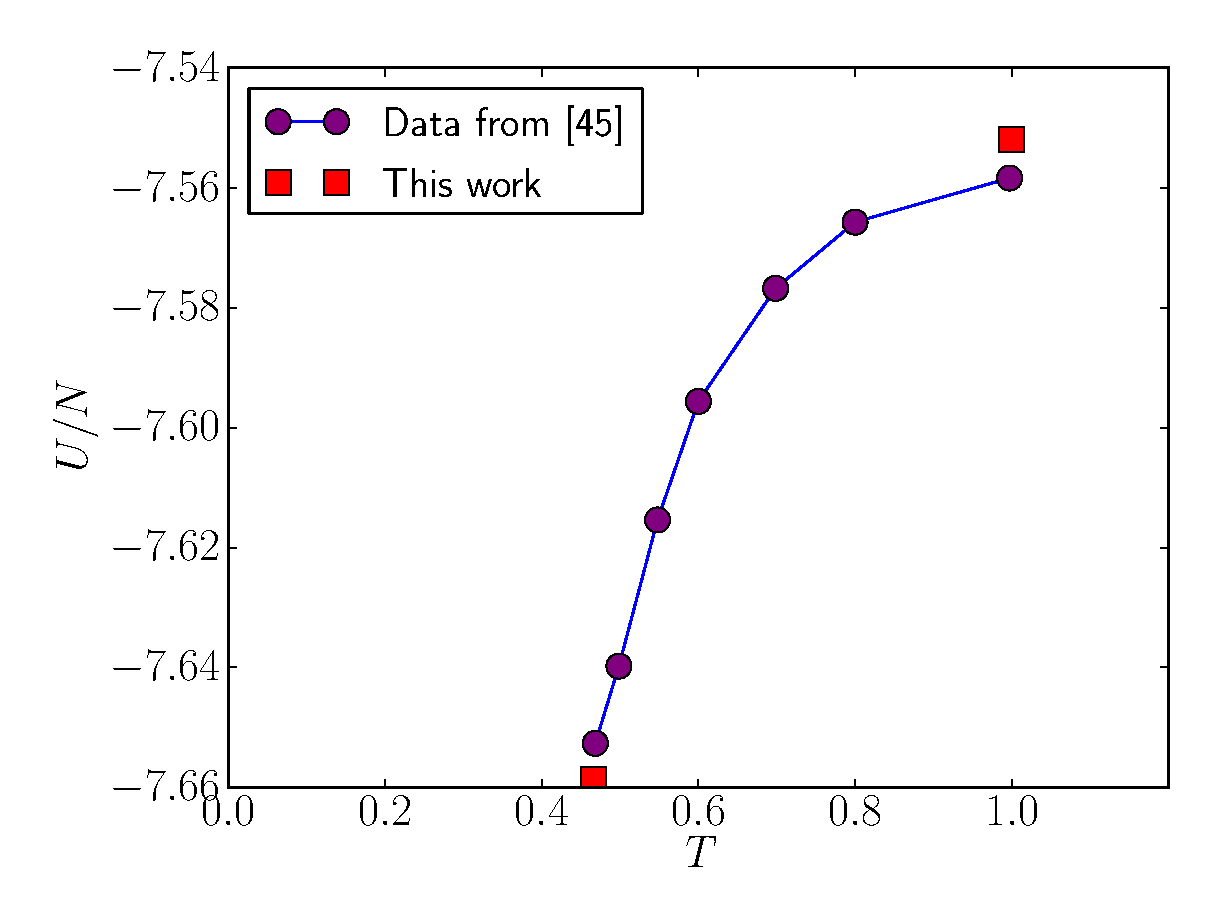
\includegraphics[width=0.8\textwidth]{MyUvsT.pdf} 
\caption{Average energy per particle for inherent configurations of the KA mixture at $N=500$ for different effective temperatures. Data taken from \cite{lacks2004energy} has been extracted from \autoref{fig:UvsT}. \label{fig:MyUvsT}}
\end{figure}

In order to obtain samples differing in their features, we consider equilibrium samples at two different temperatures $T=0.466$ and $T=1.0$, compute their trajectories via an NVE protocol, take samples separated by intervals of duration $\tau_{r}$ in the NVE trajectory, neglect the velocities and minimize their energy via CG, so to obtain inherent structures whose respective effective temperature is equal to $T$. The plot \autoref{fig:MyUvsT} shows that these configurations do have significantly different average potential energies, and thus differ by their statistical properties.
These will be the starting configurations of our AQS simulations described in the paragraph below. 

\section{Results of AQS shear deformation simulations}

We take different samples of different sizes and effective temperature $T$ and we subject them to AQS oscillatory deformation for different values of $\gamma_{max}$. The value of $\delta \gamma$ must be carefully chosen, so that the modification of the landscape induced by a strain increment of $d\gamma$ is weak enough so that all the dynamics is correctly sampled (see also discussion in \autoref{sec:LJDeformation}). This condition is assumed to be satisfied if $d\gamma$ is much smaller than the typical strain interval between two consecutive transitions\footnote{In other words, the sampling resolution in the plot \autoref{fig:UVsGamma} should be less than the separation between the values of the strain }. To verify that the choice of $d\gamma$ is appropriate one can check that a choice of a smaller $d\gamma$ does produce similar dynamics. In what follows we use $d\gamma = 0.001, 0.0002, 0.0002$ for $N = 500, 4000, 32000$ respectively.
We monitor the potential energy $U$ and the components of the stress tensor $\sigma$ for every value of the accumulated strain $\gamma_{acc}$ (see \autoref{eq:AccumulatedStrain}) and record the positions of the particles at configurations such that $\gamma = 0$. 

\subsection{Energy of the structures: overaging and rejuvenation \label{sec:EnergyBehavior}}

By performing oscillatory deformation of KA samples at different effective $T$ we extend what has been performed in \cite{lacks2004energy}, and apply a large number of cycles rather than just a semicycle\footnote{Our protocol resembles that applied in \cite{duff2007shear} on crystallizing samples.}. In \cite{lacks2004energy}, by monitoring the potential energy behavior of the samples during the application of the deformation, it is noted that depending on the initial $T$ and on the amplitude of deformation semicycle samples tend either to lower their potential energy $U$, reaching deeper inherent structures (they undergo \emph{overaging}) or samples tend to reach higher $U$'s (they undergo \emph{rejuvenation}). The data presented in \cite{lacks2004energy}, however, do not say more about whether a given choice of the amplitude $\gamma_{max}$ and initial effective $T$ leads to rejuvenation and some other leads to overaging. What we show in this thesis is that the results in \cite{lacks2004energy} can be rationalized simply by increasing the number of oscillations cycles. In particular, we measure (in reduced LJ units) the potential energy per particle $U/N$ of unstrained configurations ($\gamma = 0$) for increasing $\gamma_{acc}$. 
By doing so, one gets the behavior plotted in \autoref{fig:UvsAccumulatedStrainKA} (data are relative to the particular case $N=4000$ and averaged over $\approx 10$ samples): for large enough values of $\gamma_{acc}$ (i.e. for very many oscillation cycles) after a transient $U$ tends to approach a plateau value that depends on $\gamma_{max}$, is independent from the initial effective $T$, and increases with higher $\gamma_{max}$. For small values of $\gamma_{max}$, $U$ reaches a plateau also, but its asymptotic value depends on both $\gamma_{max}$ and the initial effective $T$. These facts imply that:

\begin{enumerate}
	\item For high $\gamma_{max}$, whether a sample at effective temperature $T$ will undergo overaging or rejuvenation depends on whether the initial $U(T)$ is higher or lower than the plateau value of $U$ which is reached for large $\gamma_{acc}$ by all samples deformed by cycles of amplitudes $\gamma_{max}$.
	\item For high $\gamma_{max}$, and for high enough $\gamma_{acc}$, samples at different initial effective $T$ lose memory of their initial state via oscillatory deformation, reaching states that cannot be distinguished (at least by looking at the energy $U$).
	\item For low $\gamma_{max}$, the value of $U$ at high $\gamma_{acc}$ depends on the initial $T$. In this case, one cannot make a general statement about whether rejuvenation or overaging will take a place. Still, generally speaking, small $\gamma_{max}$ will tend to overage the samples, whereas large $\gamma_{max}$ will tend to rejuvenate them, and samples with low effective $T$ will tend more easily to rejuvenate than those with a higher effective $T$.
	\item For low $\gamma_{max}$, samples retain memory of their initial $T$, even for high values of $\gamma_{acc}$.
\end{enumerate}

\begin{figure}[!h] 
\centering 
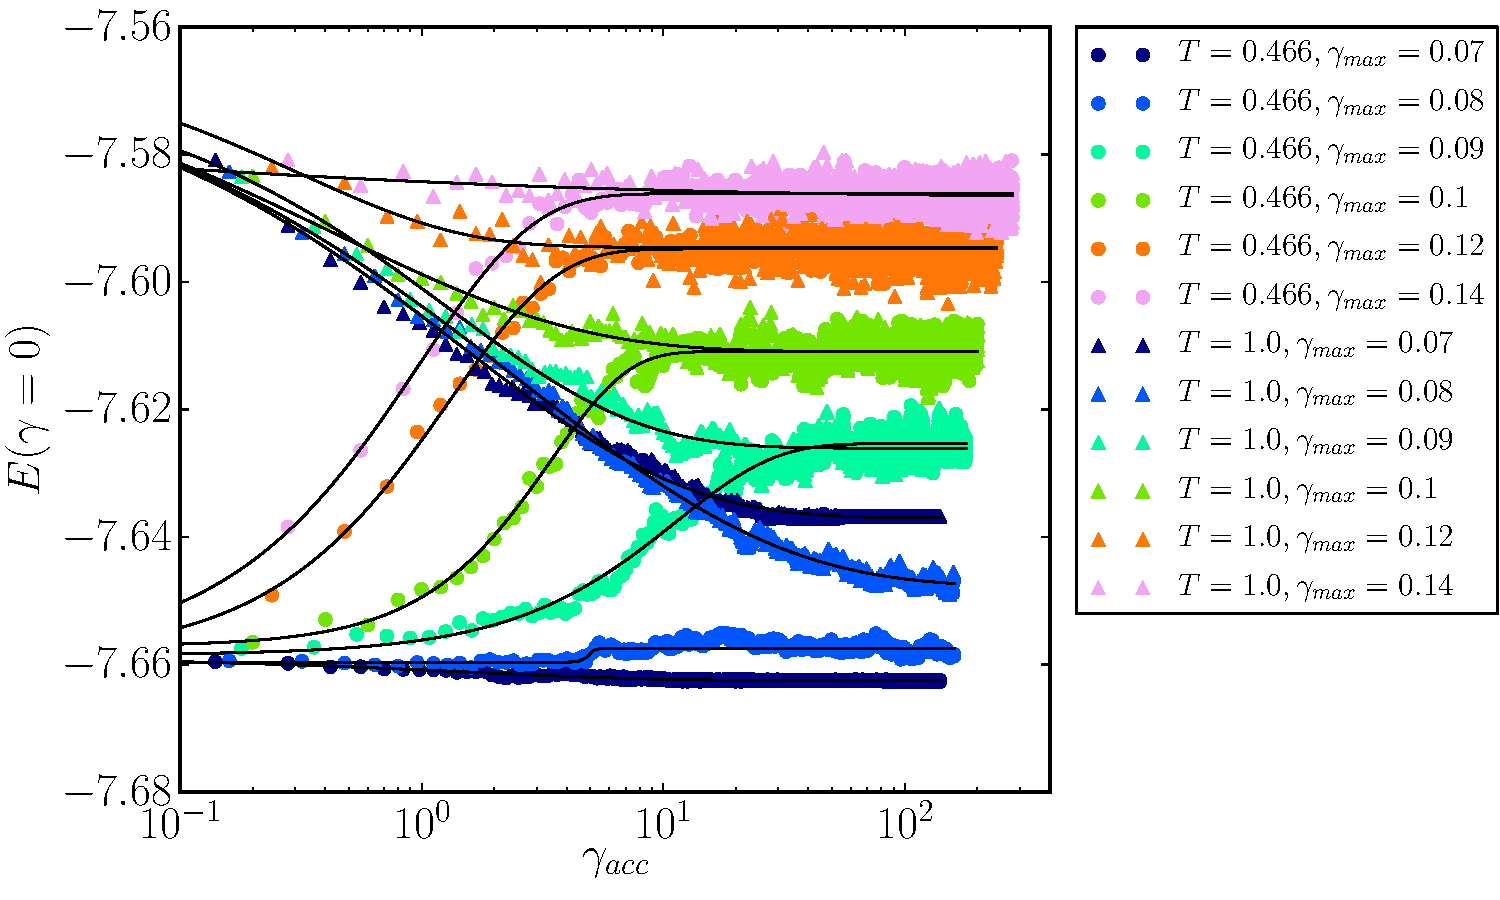
\includegraphics[width=0.9\textwidth]{EKA4000.pdf} 
\caption{Potential energy per particle $U/N$ as a function of $\gamma_{acc}$, for different initial effective temperatures and different deformation amplitudes $\gamma_{max}$ and averaged over $\approx 10$ sample realizations. The sizes of the considered systems is $N=4000$, and the data refer to configurations with $\gamma = 0$. Fits using \autoref{eq:StretchedExponentialU}. For low values of $\gamma_{max}$, the average energy assumes a fixed value beyond some characteristic $\widetilde{\gamma}_{acc}$, which depends both on $\gamma_{max}$ and on the initial effective temperature. For large values of $\gamma_{max}$ the energy fluctuates around some value which depends on $\gamma_{max}$ only. Approximatively, small $\gamma_{max}$ correlate with overaging and large $\gamma_{max}$ are associated with rejuvenation, as in \cite{lacks2004energy}. \label{fig:UvsAccumulatedStrainKA}}
\end{figure}

Note that the results in \cite{lacks2004energy} can be viewed as a transient of the curves plotted in \autoref{fig:UvsAccumulatedStrainKA}. In fact, as just a single semicycle is performed in \cite{lacks2004energy}, results in \cite{lacks2004energy} correspond to our data at $\gamma_{acc} = 2\gamma_{max}$. Overaging or rejuvenation in \cite{lacks2004energy} is thus the very beginning of the approach to a plateau value which is associated to $\gamma_{max}$ only (for $\gamma_{max}$ high enough) or to $\gamma_{max}$ and $T$ (for lower values of $\gamma_{max}$).

\subsubsection{Relaxation behavior of the energy curves under deformation}

The potential energy trends as a function of $\gamma_{acc}$ are curves approaching an asymptote for large values of $\gamma_{acc}$. We thus try to fit the $U$ data using a stretched exponential model of the form
\begin{equation}
	U(\gamma_{acc}) = (U(0) - U(\infty)) e^{- (\gamma_{acc} / \widetilde{\gamma}_{acc})^{\alpha}} + U(\infty){}
	\label{eq:StretchedExponentialU}
\end{equation}
The choice of such a model is justified by the fact that we're dealing with a decay behavior. The stretching exponent $\alpha$ is introduced to approximately take into account the fact that by increasing $\gamma_{acc}$ samples do travel in different regions of the landscape which change as $\gamma_{acc}$ increased, each with a characteristic $\widetilde{\gamma}_{acc}$. The fitting curves are superimposed to the data in \autoref{fig:UvsAccumulatedStrainKA}. Note how the curves reach a plateau faster for higher values of $\gamma_{max}$, meaning that at larger oscillation amplitudes a lesser number of cycles is needed to make samples relax. This observation can be made more quantitative by plotting the values of $\widetilde{\gamma}_{acc}$ obtained from the fits in \autoref{eq:StretchedExponentialU} against the oscillation amplitude $\gamma_{max}$. This is done in \autoref{fig:CharacteristicRelaxationStrainVsAccumulatedStrain}, where one can note that $\widetilde{\gamma}_{acc}$ is low for high and low values of $\gamma_{max}$ and peaks at intermediate values of $\gamma_{max}$.\\
Fitting the data in \autoref{fig:CharacteristicRelaxationStrainVsAccumulatedStrain} would allow to draw a similarity with what is found in \autoref{fig:TauVsGammaMax} in the case of suspensions. However, the number of points we have is not large enough to quantitatively model and fit the data. Gathering data in the region of the peak requires to perform AQS simulations whose duration scales with $\widetilde{\gamma}_{acc}$, and can thus become prohibitively long close to the region where $\widetilde{\gamma}_{acc}$ has a large value.

\begin{figure}[!h] 
\centering 
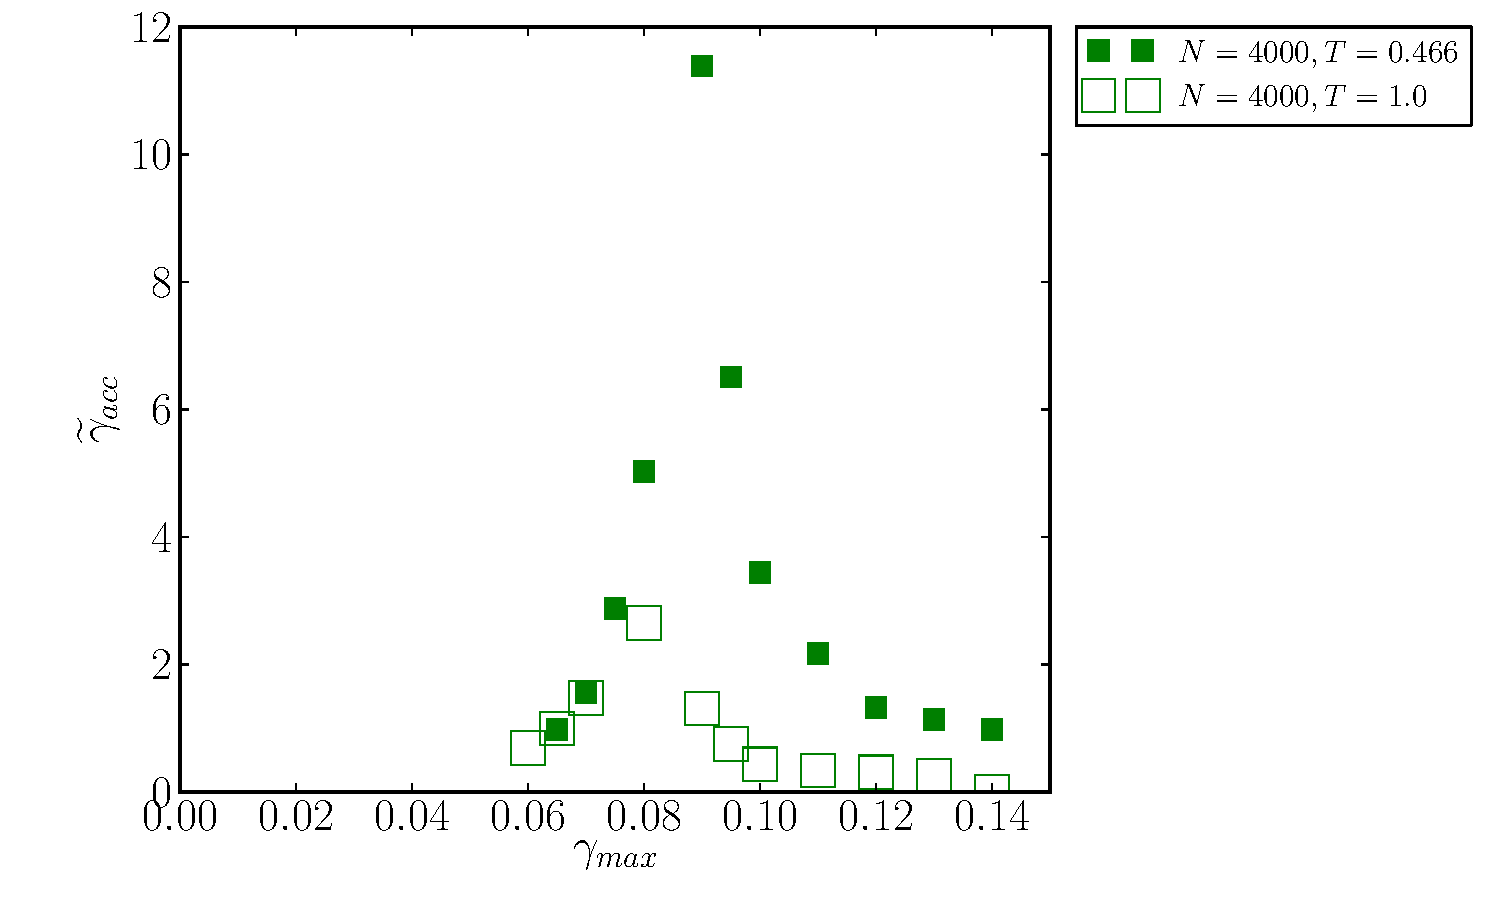
\includegraphics[width=0.9\textwidth]{Epeaks.pdf} 
\caption{Plot of the characteristic accumulated strain $\widetilde{\gamma}_{acc}$, extracted from the fits of $U$ with the stretched exponential curves in \autoref{fig:UvsAccumulatedStrainKA}, for different values of $\gamma_{max}$. The two curves look different for different effective $T$, but do both show a marked increase for intermediate values of $\gamma_{max}$ ($\approx 0.08$). \label{fig:CharacteristicRelaxationStrainVsAccumulatedStrain}}
\end{figure}

Two aspects of the energy behavior remain somewhat unexplained by the analysis of the energy data in \autoref{fig:UvsAccumulatedStrainKA} and \autoref{fig:CharacteristicRelaxationStrainVsAccumulatedStrain}. First, even though for both high and low values of $\gamma_{max}$ samples evolve to energy plateaus for a large number of oscillation cycles, the nature of the plateaus seems to be very different in the two cases: a closer inspection of \autoref{fig:UvsAccumulatedStrainKA} shows that for large values of $\gamma_{max}$ the energy fluctuates around an average value of $U$, whereas for the lowest values of $\gamma_{max}$ the potential energy reaches a \emph{fixed} value of $U$. Second, there is no indication of the mechanism that leads to the formation of a peak in the $\widetilde{\gamma}_{acc}$ plot for intermediate values of $\gamma_{max}$. These problems can be solved by looking at the motion that particles follow as a consequence of the external driving. We perform such analysis below, in \autoref{sec:DiffusionBehavior}.

\subsection{Stress tensor behavior}

The potential energy $U$ is not the sole variable that is accessible through simulations. Another quantity we examined is the stress tensor $\sigma$, which was monitored at every AQS step. \\
The stress components are defined by the expression:
\begin{equation}
	\sigma_{ij} = \frac{1}{V} \sum_{k}^{N} r_{k,i} \cdot f_{k,j}
	\label{eq:StressTensorComponent}
\end{equation}
where $r_{k,i}$ is the $i$ coordinate of the position vector of particle $k$, and $f_{k,j}$ is the $j$ component of the total force acting on particle $k$. As the system is athermal, there is no kinetic contribution to the stress tensor.

Rather than plotting each component of $\sigma$ as a function of $\gamma_{acc}$, in \autoref{fig:EStressScatterPlotMatrix} we draw the scatter plots of the components of $\sigma$ and the potential energy $U$ for high values of $\gamma_{max}$. Data are relative to samples with $N=4000$ and  with $\gamma = 0$, and are parametric plots of $\gamma_{acc}$.

\begin{figure}[!hp] 
\centering 
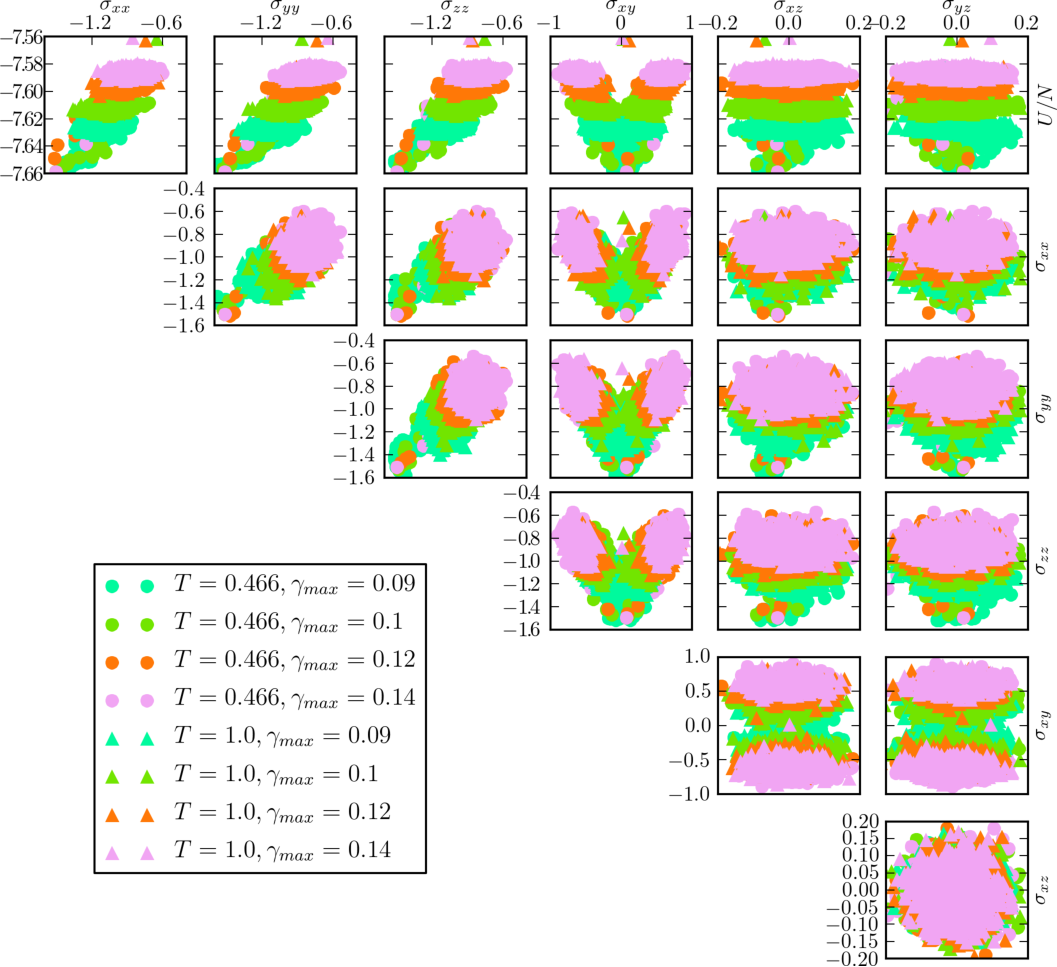
\includegraphics[width=\textwidth]{EsigmaMatrix-4000.pdf} 
\caption{Matrix of scatter plots of $\sigma_{ij}$ and $U$, which both depend parametrically on $\gamma_{acc}$, for different (and large) values of $\gamma_{max}$ and initial effective temperatures $T$, in samples with $N=4000$. Data are all relative to $\gamma=0$, so that the stress components are all \emph{residual} stress components. The ``blobs'' correspond to points obtained where the majority of data fall, which is the steady state. Outliers refer to points collected at the very beginning of the deformation oscillations. 
The ensemble of plots indicates that samples with different effective temperatures do assume the same values of $U$ and $\sigma_{ij}$ in the steady state if they are sheared with the same amplitude $\gamma_{max}$ (as triangle and circles of the same color overlap in the blobs).
From the first row of scatter plots, it's clear that an increase of $\gamma_{max}$ corresponds to a higher potential energy $U$, increasing values of the diagonal values of the stress $\sigma_{ii}$ and an increasing shear stress in the plane of deformation $\sigma_{xy}$. In particular, the residual stress $\sigma_{xy}$ is also seen oscillating between negative and positive values (whose absolute value increases as $\gamma_{max}$ is increased), depending on the direction of the deformation. The dependence of $U$ from $\sigma_{ii}$ and $\sigma_{xy}$ seems approximately linear.
From the plot of $\sigma_{xz}$ against $\sigma_{yz}$ one sees that these components of the stress tensor are basically unaffected by the deformation. \label{fig:EStressScatterPlotMatrix}}
\end{figure}

All the scatter plots in \autoref{fig:EStressScatterPlotMatrix} are parametric in $\gamma_{acc}$, so that each point in them represents a value of $U$ and/or a component of $\sigma$ at a different value of $\gamma_{acc}$ (multiple of $4\gamma_{max}$). \autoref{fig:EStressScatterPlotMatrix} contains a lot of information. One of these is that large oscillation amplitudes make all components of $\sigma$ and $U$ converge to a common value that depends on $\gamma_{max}$, regardless the initial effective $T$ of the samples. This is clear from the fact data relative to two different initial temperatures $T$ all fall into the same ``blobs'' in the steady state if they are associated to a common $\gamma_{max}$. As for the steady state, large $\gamma_{max}$ oscillations do bring systems to configuration of higher $U$ and residual $\sigma_{xx}$, $\sigma_{yy}$, $\sigma_{zz}$ and $\sigma_{xy}$ (the shear stress on the plane of deformation), whereas $\sigma_{xz}$ and $\sigma_{yz}$ seem unaffected by the deformation. The relationship between $U$ and the diagonal components of the stress and $\sigma_{xy}$ appears to be approximately linear (see first row of panels), but our data does not allow a very precise determination of the functional form \cite{bouchbinder2013private}. 

\subsection{Diffusion behavior \label{sec:DiffusionBehavior}}

To quantify particle motion we first measure the mean squared displacement (MSD) of the sample from the initial configuration $\mathbf{R}(0)$ for increasing values of $\gamma_{acc}$, for samples with $N=4000$ such that $\gamma = 0$:
\begin{equation}
	\text{MSD} (\gamma_{acc}) = \frac{1}{N} \sum_{i}{(\mathbf{r_{i}}(\gamma_{acc}) - \mathbf{r_{i}}(0))^{2}}
	\label{eq:MSD0VsAccumulatedStrain}
\end{equation} 
The result is plotted in \autoref{fig:MSD0VsAccumulatedStrain}. Depending on $\gamma_{max}$ the behavior of the MSD is strikingly different: for low values of $\gamma_{max}$ the MSD saturates to a finite value, whereas for higher values it behaves linearly. 

\begin{figure}[!h] 
\centering 
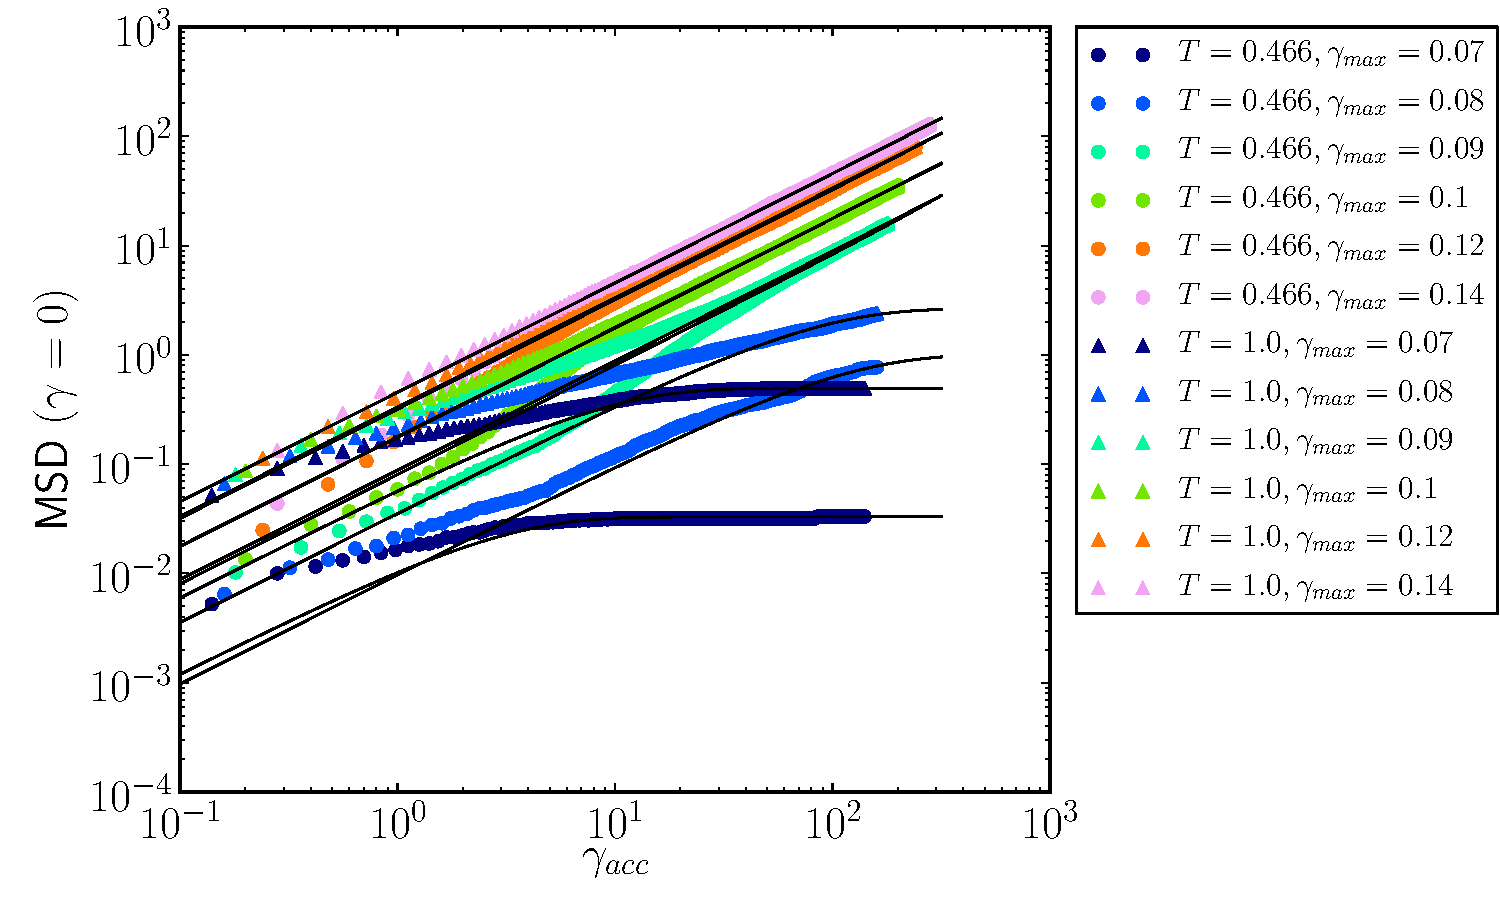
\includegraphics[width=0.8\textwidth]{MSDKA4000.pdf} 
\caption{Mean squared displacement as a function of $\gamma_{acc}$, for different initial effective temperatures and different deformation amplitudes $\gamma_{max}$, measured from the initial undeformed configuration and averaged over several samples with $N=4000$ particles. For low $\gamma_{max}$, after a transient the systems do stop moving, and the respective MSD reaches a plateau. For larger values of $\gamma_{max}$, the systems are diffusive. This behavior can be descibed with the mortal random walk model in \autoref{eq:MortalRandomWalkMSD} (black curves), but the fits are not completely satisfying. \label{fig:MSD0VsAccumulatedStrain}}
\end{figure}

Such behavior is remarkable: samples below some value of $\gamma_{max}$ at some point do stop their motion in configuration space, whereas if $\gamma_{max}$ is high enough samples get farther and farther from the initial configuration. In the first case a system reaches a state that is a sort of ``trap'' which is stable under an oscillation of amplitude $\gamma_{max}$. The nature of such traps (named ``absorbing'' states) is explored in more detail in \autoref{ch:Memory}.
The observation of such transition in the dynamics resolves one of the issues raised during the observation of the potential energy trends: oscillations at low values of $\gamma_{max}$ reach a fixed value of $U$ just because samples do cease to travel in configuration space. 

In order to interpret the data in \autoref{fig:MSD0VsAccumulatedStrain} one can assume that systems diffuse in configuration space like random walkers in $3N$D as a consequence of deformation. Their diffusion constant is $D$, and can they stop permanently their motion with a probability $\lambda$ per unit $\gamma_{acc}$. The details of such a ``mortal random walk'' model (recently explored also in \cite{yuste2013exploration}) are given in \autoref{app:MortalRandomWalk}. Within such a model the MSD can be expressed as 
\begin{equation}
	\text{MSD} (\gamma_{acc}) =  \frac{D}{\lambda N} (1 - e^{-\lambda \gamma_{acc}})
	\label{eq:MortalRandomWalkMSD}
\end{equation} 
where $D$ is $\gamma_{max}$ dependent. In fact, it's reasonable to assume that higher values of $\gamma_{max}$ will make the sample undergo longer leaps in configuration space\footnote{This is because the larger the oscillation amplitudes, the larger are the probabilities for the system to ``get lost'' in configuration space and find itself displaced from the initial configuration after a full oscillation cycle.}. The parameter $\lambda$ is also expected to be dependent on $\gamma_{max}$, as for higher oscillation amplitudes fewer points of configuration space will be able to act as ``traps''. As the density of such states in configuration space is lower, so will be the likelihood to encounter them.
Fits obtained using the expression in \autoref{eq:MortalRandomWalkMSD} varying $D$ and $\lambda$ are plotted for different data series in \autoref{fig:MSD0VsAccumulatedStrain}. The quality of the fits is not excellent, possibly because the dynamics of the system depends on the features of the landscape explored by the system. These change as $\gamma_{acc}$ is increased: this can be seen, for instance, in \autoref{fig:UvsAccumulatedStrainKA}, where the average $U$ of the configurations explored by the system depends on $\gamma_{acc}$ until a plateau is reached. If $U$ changes with $\gamma_{acc}$, so will the landscape. It is thus reasonable to assume that $D$ and $\lambda$ will change as well as $\gamma_{acc}$ increases.
In other words, the partial failure of the mortal random walk model can be attributed to the initial transient that the system experiences at low number of oscillation cycles. \\
An alternative approach to describe particle motion is to exclude from the analysis the transient altogether, and study the MSD of the system starting from a reference configuration at a value of $\gamma_{acc}$ such that a ``steady'' state has already been attained. For instance one can measure the MSD starting from the state visited at $\widetilde{\gamma}_{acc}$, as determined from the fits of the energy trends of the kinds shown in \autoref{fig:UvsAccumulatedStrainKA}:
\begin{equation}
	\text{MSD} (\gamma_{acc} - \widetilde{\gamma}_{acc}) = \frac{1}{N} \sum_{i}{(\mathbf{r_{i}}(\gamma_{acc}) - \mathbf{r_{i}}(\widetilde{\gamma}_{acc}))^{2}}
	\label{eq:MSDVsAccumulatedStrain}
\end{equation} 
Plots of the MSD obtained this way are shown in \autoref{fig:MSDVsAccumulatedStrain} and are much easier to interpret: for low $\gamma_{max}$ systems simply do not move, so their $\text{MSD} (\gamma_{acc} - \widetilde{\gamma}_{acc})$ is close to zero, whereas for higher $\gamma_{max}$ the MSD increases linearly, with no samples seeming to reach absorbing states within our range of $\gamma_{acc}$. One can thus simply write:
\begin{equation}
	\text{MSD} (\gamma_{acc} - \widetilde{\gamma}_{acc}) =  D (\gamma_{acc} - \widetilde{\gamma}_{acc})
	\label{eq:DiffusiveMSD}
\end{equation}
Linear fits are superimposed to the data in \autoref{fig:MSDVsAccumulatedStrain}.

\begin{figure}[!h] 
\centering 
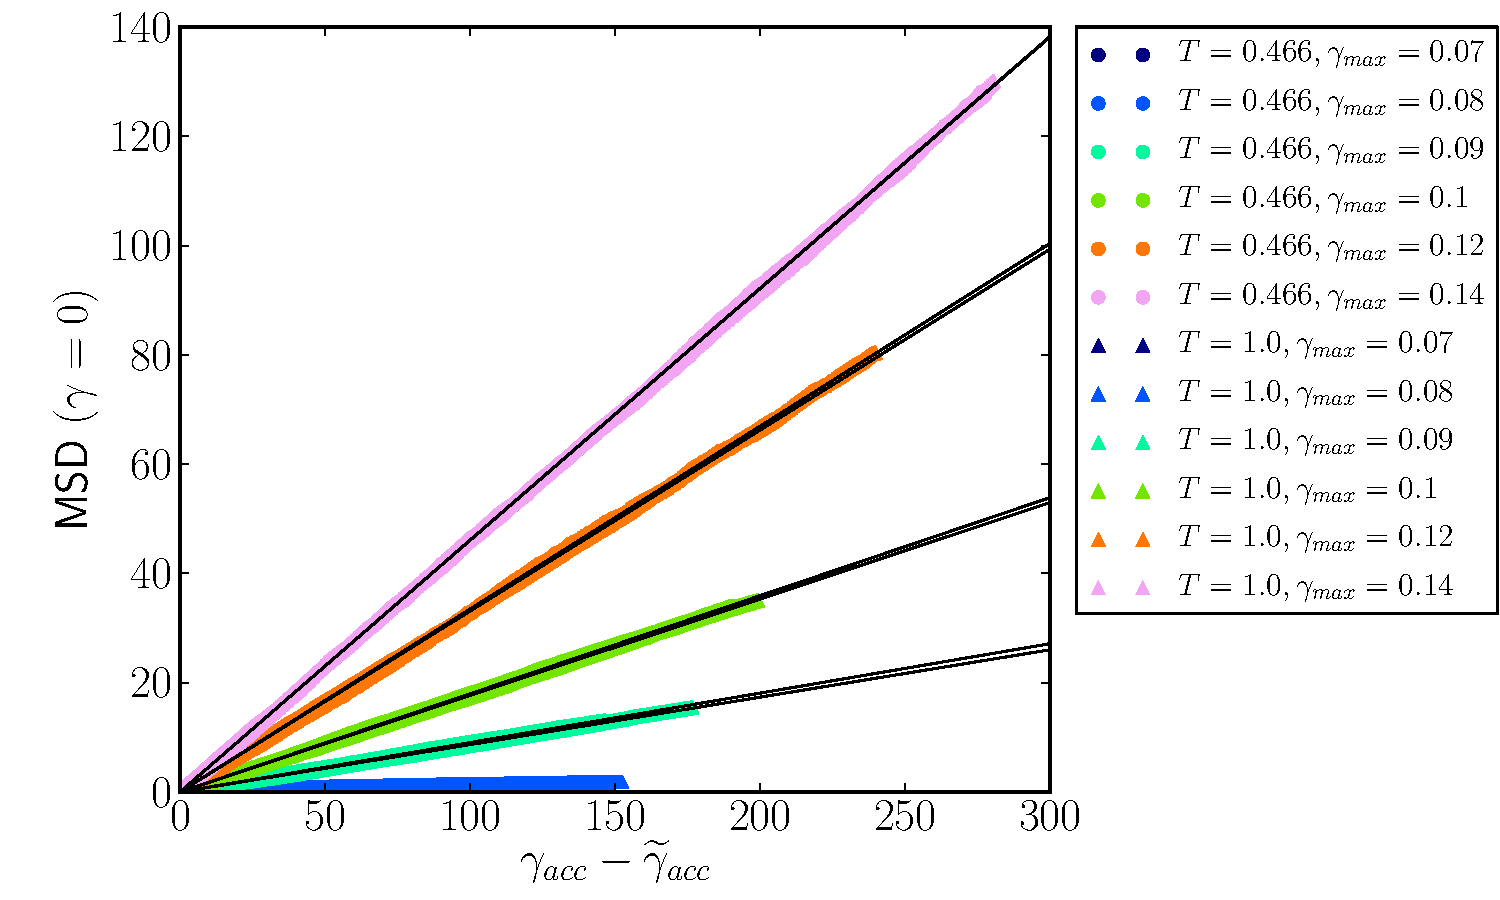
\includegraphics[width=0.8\textwidth]{MSDRelaxKA4000.pdf} 
\caption{Mean squared displacement as a function of $\gamma_{acc} - \widetilde{\gamma}_{acc}$, for different initial effective temperatures and different deformation amplitudes $\gamma_{max}$, measured from configurations such that $\gamma=0$ and $\gamma_{acc} > \widetilde{\gamma}_{acc}$. For low $\gamma_{max}$, the systems don't move, and their respective MSD is 0. For larger values of $\gamma_{max}$ instead the systems are diffusive. This allows to fit the data with the model in \autoref{eq:DiffusiveMSD} (black curves). The diffusion constant depends on $\gamma_{max}$ only, and not on the effective $T$ of the samples.
\label{fig:MSDVsAccumulatedStrain}}
\end{figure}

Data series obtained from samples at different effective $T$ do overlap, showing that after the transient systems reach states having an equivalent behavior in terms of particle motion.

\begin{figure}[!h] 
\centering 
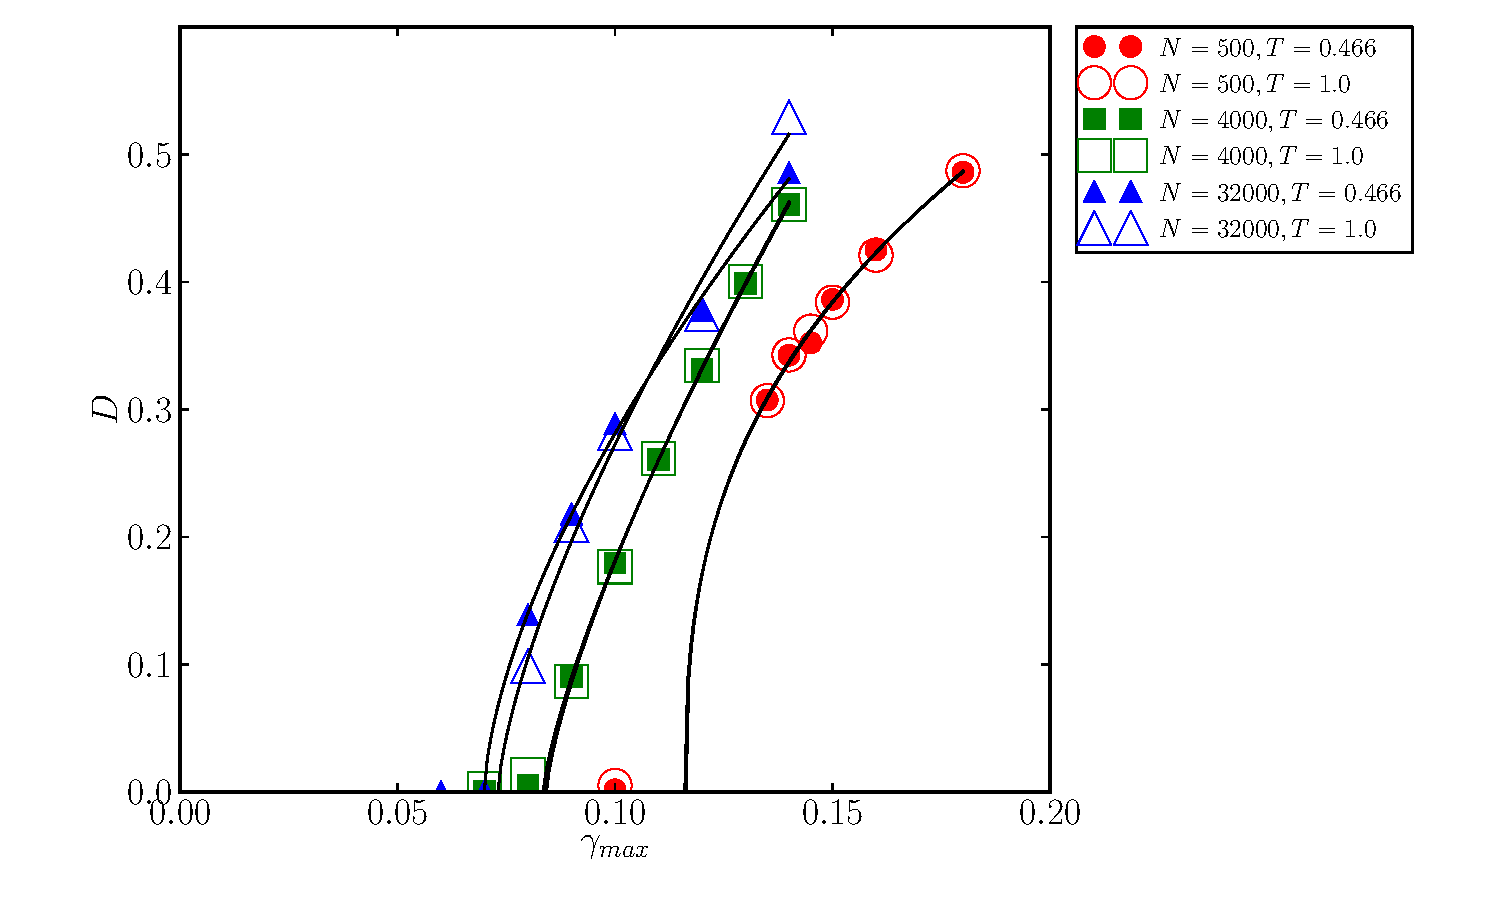
\includegraphics[width=0.8\textwidth]{D.pdf} 
\caption{Diffusion constant of the model \autoref{eq:DiffusiveMSD} determined from fits as those in \autoref{fig:MSDVsAccumulatedStrain} as a function of $\gamma_{max}$, for different system sizes. $D$ seems in all cases to become non-zero at a value $\gamma_{c}$, which depends on the system size. Data can be described approximately with a power law (\autoref{eq:DPowerLaw}, black curves). \label{fig:DVsGammaMax}}
\end{figure}
The linear fits of $\text{MSD} (\gamma_{acc} - \widetilde{\gamma}_{acc})$ allow to study the way $D$ depends on $\gamma_{max}$, and from \autoref{fig:DVsGammaMax} one can see how particle motion under oscillatory strain depends crucially on the oscillation amplitude for the class of systems under consideration. This is one of the main results of this thesis and the main result in \cite{fiocco2013oscillatory}. For low $\gamma_{max}$ $D$ is zero and at some value of the amplitude (which we will refer to as ``critical'' $\gamma_{c}$), systems increase their MSD in \autoref{eq:DiffusiveMSD} linearly. The values of $D$ can be fitted by a power law of the form
\begin{equation}
	D = A (\gamma_{max} - \gamma_{c})^{\beta}. 
	\label{eq:DPowerLaw}
\end{equation}

The values of $\gamma_{c}$ as determined via the fits are dependent on the sizes of the systems, with $\gamma_{c}$ decreasing for increasing $N$. This raises the doubt that $\gamma_{c}$ could be an artifact of out simulations and thus vanish in the limit $N \rightarrow \infty$. To check if this is the case we plot in \autoref{fig:CriticalGammaVsInverseSize} the values of $\gamma_{c}$ against the inverse system size. An analysis of \autoref{fig:CriticalGammaVsInverseSize} seems to exclude this scenario, even though our data points are too few to completely rule out the possibility of a sharp turn in the $\gamma_{c}$ dependence at low $1/N$ such that $\gamma_{c} \rightarrow 0$ for large $N$.

\begin{figure}[!h] 
\centering 
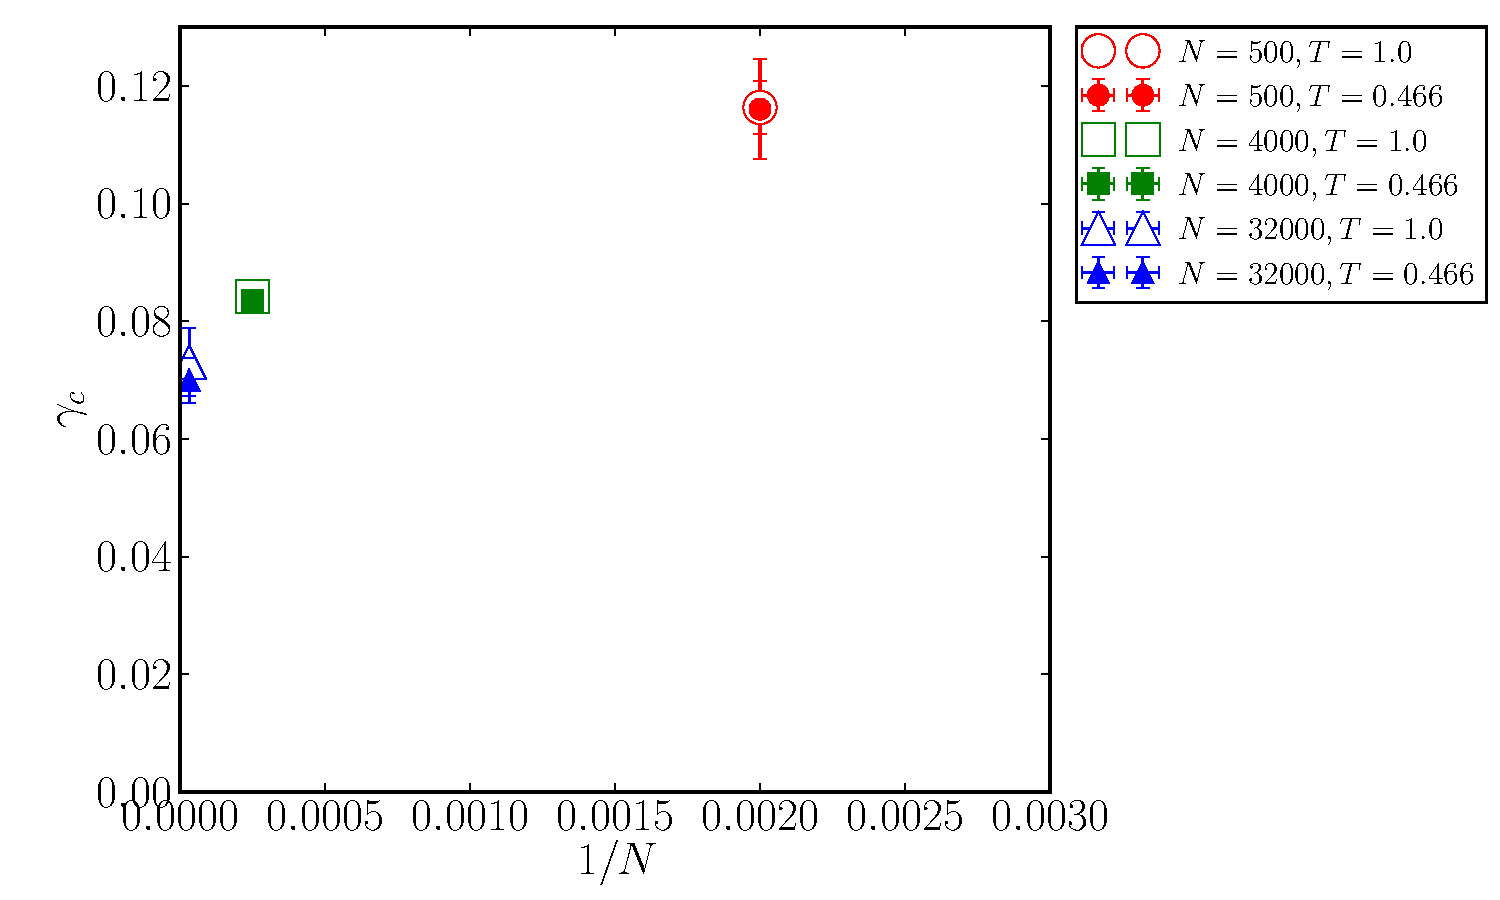
\includegraphics[width=0.8\textwidth]{GammacScaling.pdf} 
\caption{Values of $\gamma_{c}$ determined from the fits in \autoref{fig:DVsGammaMax} as a function of the inverse system size. $\gamma_{c}$ is lower at larger $N$, but our data tend to suggest that $\gamma_{c}$ will be non-zero in the limit $N \to \infty$. \label{fig:CriticalGammaVsInverseSize}}
\end{figure}

The values of $\beta$ in \autoref{eq:DPowerLaw} obtained from the fits in \autoref{fig:DVsGammaMax} are reported in \autoref{tab:Beta}. Such values seem not to be compatible with the exponent $\beta = 0.84$ which pertains to conserved directed percolation in 3D \cite{menon2009universality}, so our model does not seem to fit in this non-equilibrium universality class \cite{hinrichsen2000nonequilibrium}. However, more precise estimates of $\beta$ (through better statistics on the data in \autoref{fig:DVsGammaMax} and a precise estimate of size effects) would be needed to conclusively confirm this.

\begin{table}
	\centering
	\begin{tabular}{| c | c | c |}
		$N$ & $\beta$ \\
		\hline 
		$500$ & $0.37 \pm 0.11$ \\
		$4000$ & $0.74 \pm 0.08$ \\
		$32000$ & $0.69 \pm 0.11$ \\
		\hline 
	\end{tabular}
	\caption{Average values of the exponents $\beta$ obtained from the fits of the data in \autoref{fig:DVsGammaMax} as a function of the size of the systems. \label{tab:Beta}}
\end{table}

For the system sizes studied, $\gamma_{c}$ seems to have a crucial role and separates two regimes, so that the data in \autoref{fig:MSD0VsAccumulatedStrain}, \ref{fig:MSDVsAccumulatedStrain}, \ref{fig:CriticalGammaVsInverseSize} and especially the peak of $\widetilde{\gamma}_{acc}$ in \autoref{fig:CharacteristicRelaxationStrainVsAccumulatedStrain} can be interpreted in the following way:
\begin{itemize}
	\item For $\gamma_{max} \ll \gamma_{c}$: Due to the low value of $\gamma_{max}$, the undeformed ($\gamma_{acc} = 0$) system initially travels slowly in configuration space, but soon reaches an absorbing state. This is because there's a large number of states in configuration space that can act as traps for the system if it falls in one of them. For these reasons, the value of $\widetilde{\gamma}_{acc}$ extracted from the fits of the potential energy is low and the MSD (computed with the expression in \autoref{eq:MSD0VsAccumulatedStrain} and plotted in \autoref{fig:MSD0VsAccumulatedStrain}) saturates at correspondingly low values of $\gamma_{acc}$.
	\item For $\gamma_{max} < \gamma_{c}$: A higher amplitude means a faster exploration of configuration space, but the number of states that are absorbing is severely reduced as $\gamma_{max}$ approaches $\gamma_{c}$, so that $\widetilde{\gamma}_{acc}$ becomes increasingly high, and the MSD takes a correspondingly large value of $\gamma_{acc}$ to saturate. 
	\item For $\gamma_{max} > \gamma_{c}$: Virtually no absorbing states exist above $\gamma_{c}$ so that the MSD can't saturate. The exploration of configuration space is still not very fast, so that the transient in the energy $U$ lasts long ($\widetilde{\gamma}_{acc}$ high). The MSD is linear when calculated with both \autoref{eq:MSD0VsAccumulatedStrain} and \autoref{eq:MSDVsAccumulatedStrain}.
	\item For $\gamma_{max} \gg \gamma_{c}$: No absorbing states exist above $\gamma_{c}$, and the exploration of configuration space is fast. The value of $\widetilde{\gamma}_{acc}$ is thus low, and the MSD is linear with a steep slope.
\end{itemize}

\subsubsection{Nature of the absorbing and ``diffusive'' states, ``shear banding''}

The MSD computed with \autoref{eq:MSD0VsAccumulatedStrain} and \autoref{eq:MSDVsAccumulatedStrain} gives an average isotropic measure of particle motion of deformed systems. But it does not say, for instance, if particles do move preferentially in some direction rather than others, or if some particles move more than others when samples are subjected to oscillatory deformation. \\
Inspection of the displacement of the particles does show that the distribution of particles that move the most can be spatially inhomogeneous. In \autoref{fig:ShearBands} we plot configurations of particles at $\gamma = 0$ which have reached the steady state for oscillatory deformation of $\gamma_{max} > 0.1$, highlighting in red particles that move more than $0.8$ (in reduced units) when they are subjected to a single additional deformation cycle. In samples with $N=32000$ particles that move the most are clearly localized in a band which is parallel to the $xz$ plane and whose thickness is approximately half of the simulation box. In addition, such band doesn't change in thickness and position if it is recomputed after having applied several cycles to the sample, and its thickness is weakly dependent on $\gamma_{max}$.
Smaller samples do not show this kind of phenomenon (see for instance the $N=4000$ samples in \autoref{fig:Band4000Small} and \autoref{fig:Band4000Large}). In smaller samples the particles that move the most do correlate in space, but without giving rise to band-like structures. We thus surmise that bands observed in our largest samples could be observed in even larger samples, possibly showing the same thickness. Bands wouldn't occur in our smaller samples simply because these are smaller than the characteristic thickness of such bands. 
It would be interesting to check whether such bands exist in larger samples, and if \emph{multiple} bands can arise and interact. However, such investigation has proved to be beyond the computational power at our disposal (samples with $N > 100000$ would have required running times exceeding a month on our 48 CPU cluster nodes).

\begin{figure}
	\centering
	\begin{subfigure}[b]{0.45\textwidth}
			\centering
			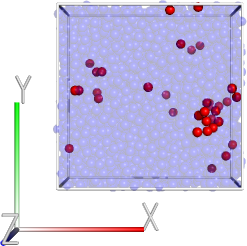
\includegraphics[width = 0.4\textwidth]{bandsN4000g010.png}
			\caption{\label{fig:Band4000Small}}
	\end{subfigure}
	\begin{subfigure}[b]{0.45\textwidth}
			\centering
			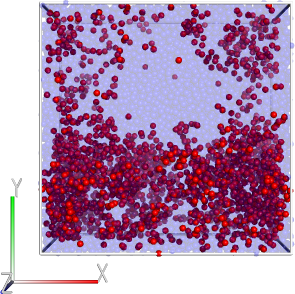
\includegraphics[width = 0.7\textwidth]{bandsN32000g010.png}
			\caption{\label{fig:Band32000Small}}
	\end{subfigure}
	\begin{subfigure}[b]{0.45\textwidth}
			\centering
			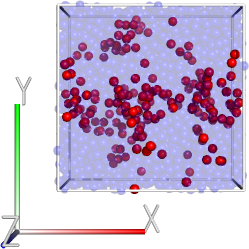
\includegraphics[width = 0.4\textwidth]{bandsN4000g012.png}
			\caption{\label{fig:Band4000Large}}
	\end{subfigure} 
	\begin{subfigure}[b]{0.45\textwidth}
			\centering
			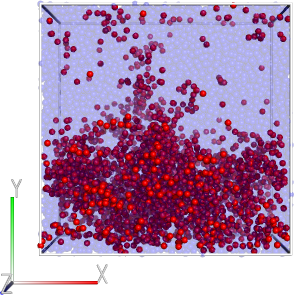
\includegraphics[width = 0.7\textwidth]{bandsN32000g012.png}
			\caption{\label{fig:Band32000Large}}
	\end{subfigure}
	\caption{Typical samples with $N=4000$, $32000$ in the steady state for oscillatory deformations of $\gamma_{max} = 0.1$ ((\subref{fig:Band4000Small}) and (\subref{fig:Band32000Small})) and 0.12 ((\subref{fig:Band4000Large}) and (\subref{fig:Band32000Large})). Particles which move more than $0.8$ (in reduced units) if the samples are subjected to an additional cycle are highlighted in red. Clearly such particles are organized in bands in the largest samples, whereas no such spatial heterogeneity is visible in the smaller samples.
	\label{fig:ShearBands}}
\end{figure}

%\subsubsection{Normal modes of the structures in the steady state}
%
%One of the issues that is addressed in \cite{lacks2004energy} is whether the features of samples that have undergone a single semicycle of deformation of amplitude $\gamma_{max}$ resemble those of inherent structures of equilibrium states at some temperature $T$. Such question is important because if that was the case, deformation could be a means to drive the system towards states that can be obtained in a completely different way, that is simply by quenching from some temperature $T$. In this way, a sort of equivalence between inherent structures at an effective temperature $T$ and samples having undergone deformation up to $\gamma_{max}$ could be established.
%In \cite{lacks2004energy}, the authors show that this is not the case, and that deformed states are distinguishable from equilibrium states, for instance by means of normal modes analysis. It remains however open the question whether samples that have been subjected to a high number of oscillation cycles bear a closer resemblance to inherent structures obtained from equilibrium states.

\subsection{Energy dissipation\label{sec:DissipationBehavior}}

When LJ samples are deformed by means of AQS deformation, they change their energy as a consequence of the deformation of the landscape. Most of the time energy changes are continuous, but sometimes abrupt changes due to collisions with saddle points in the energy landscape occur (see discussion in \autoref{sec:AQSDynamics} and \cite{maloney2006amorphous}). In particular, if one looks at the potential energy $U$ as a function of $\gamma$ during cyclic deformation of an inherent structure (\autoref{fig:UVsGamma}), the behavior for small amplitudes is to a first approximation elastic, with the potential energy depending quadratically from the strain $\gamma$. In fact, incrementing the strain of an initially undeformed sample has usually the effect of increasing smoothly its potential energy, so that energy is pumped into the system if the strain is increased by some amount $d\gamma$. If the sample is sheared back, it goes back spontaneously to the configuration assumed before deformation, so that no additional energy is required to bring the system to the initial state.
However, this is not always the case: by looking closely at the $U$ vs $\gamma$ curves in \autoref{fig:UVsGamma} one can see small discontinuities in $U$, due to the collisions with saddle points mentioned above. In correspondence of these, if the system is deformed it loses stability and rearranges by losing energy before finding a new stable configuration. If sheared back, it doesn't assume the configuration it had prior to the deformation, but a state with a lower energy. Additional energy is thus required to restore the original state, and some energy is thus \emph{dissipated} in the process. 

\begin{figure}[!h] 
\centering 
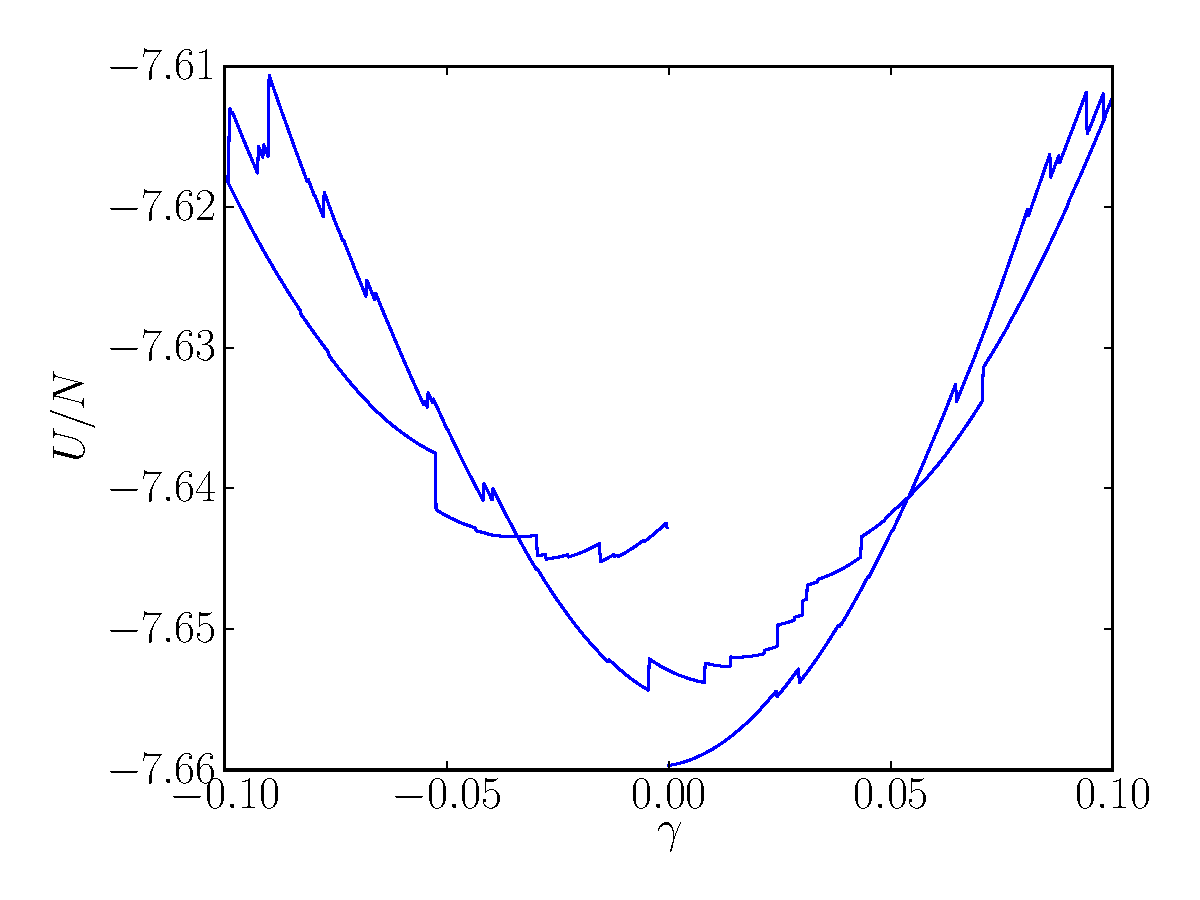
\includegraphics[width=0.7\textwidth]{SingleCycleEKA4000.pdf} 
\caption{Energy per particle as a function of the strain $\gamma$ for a sample of $N=4000$ starting from an undeformed sample. The curve shows a large number of discontinuities, each of which corresponds to a transition due to a collision with a saddle point of the energy landscape in the course of deformation. After the full cycle the system has not the same potential energy it had before the cycle, because the deformation has modified its structure. \label{fig:UVsGamma}}
\end{figure}

Rearrangements and dissipation appear more frequent as $\gamma_{max}$ is increased (this is because the system can't store arbitrarily large amounts of potential energy elastically, and rearrangements are the mechanism to release it). To quantify dissipation as a function of $\gamma_{max}$, one could simply measure the $U$ drops that occur during a cycle. An alternative, more intuitive way to do this, is to look at the behavior of the stress tensor component in the same plane of the deformation $\sigma_{xy}$ (see \autoref{eq:StressTensorComponent}) as a function of $\gamma$. The area inside the curve $\sigma_{xy}(\gamma)$ correlates\footnote{The area inside the $\sigma_{xy}$ curve is not \emph{all the work} performed on the system, because other work is performed related to variation of the other stress components.} with the work done on the system during deformation. For small values of $\gamma$, $\sigma_{xy}$ is linear in $\gamma$, and deviates from linearity at higher $\gamma$. The linearity of $\sigma_{xy}$ is required to make work linear in $\gamma$ and thus $U$ quadratic in $\gamma$. When $U$ undergoes energy drops as a consequence of rearrangements, its derivative often also has a drop, leaving a mark in $\sigma_{xy}$, which is thus sublinear \autoref{fig:SigmaVsGamma}.

\begin{figure}[!h] 
\centering 
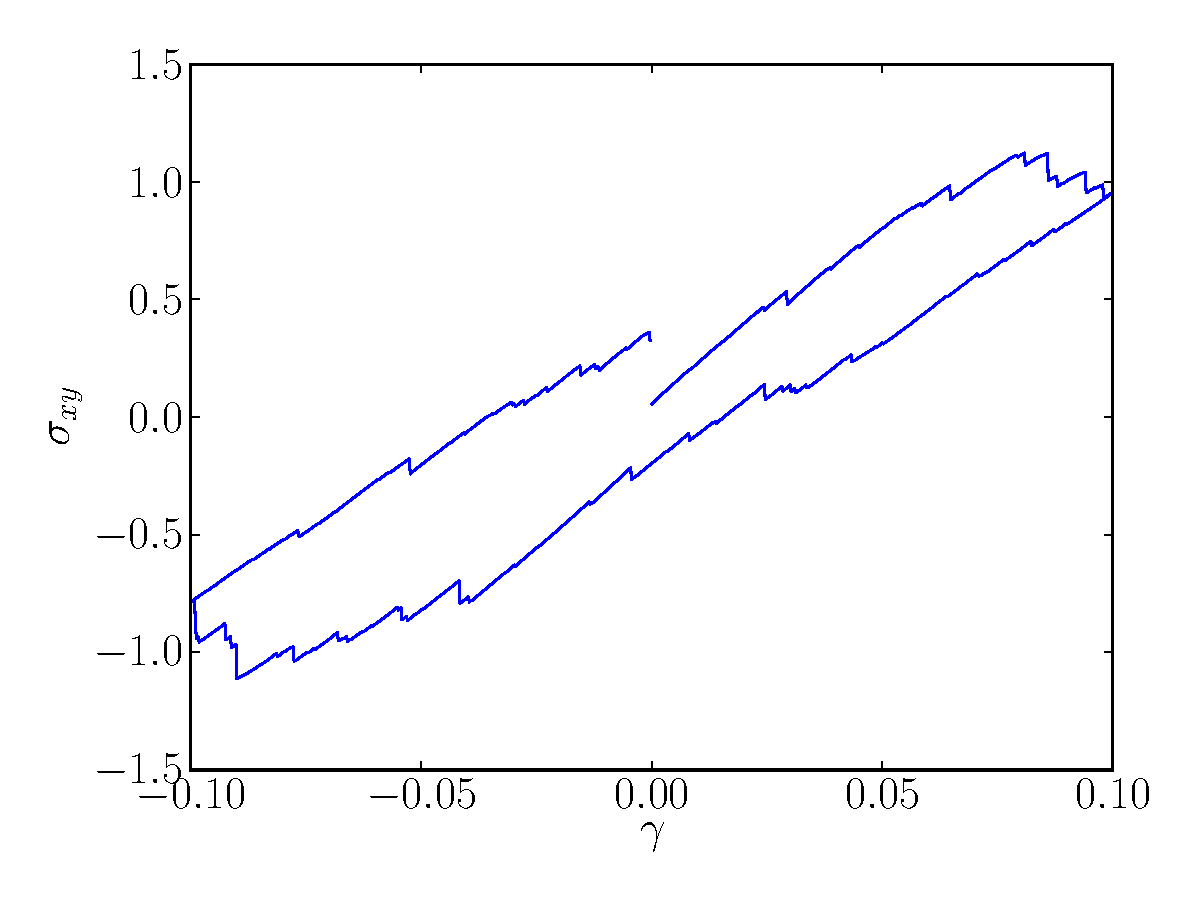
\includegraphics[width=0.7\textwidth]{SingleCycleSigmaKA4000.pdf} 
\caption{As in \autoref{fig:UVsGamma}, but plotting the stress component on the plane of the deformation rather than the energy. Again, the stress drops reflect transitions, and the fact that the stress values at the beginning and at the end of the cycle are different indicates that the sample has been modified by the deformation. \label{fig:SigmaVsGamma}}
\end{figure}

The area of the $\sigma_{xy}(\gamma)$ curve in a full cycle is thus related to the work done by the system to complete a full cycle. In the steady state mentioned in \autoref{sec:EnergyBehavior} and \autoref{sec:DiffusionBehavior}, after a full cycle the samples return to states which are \emph{statistically} similar to the initial one (for instance, $U$ is on average unchanged, by definition of steady state). This means that the work done on the system is a good measure of the dissipated energy. 
In order to measure it, we plot in \autoref{fig:Hysteresis} the $\sigma_{xy}$ hysteresis curves for different values of $\gamma_{max}$, averaged on several cycles. Hysteresis curves are very narrow and almost linear for small $\gamma_{max}$, where only few particle rearrangements and dissipation occur. For larger $\gamma_{max}$, curves widen, showing a much higher amount of dissipation per cycle.

\begin{figure}[!h] 
\centering 
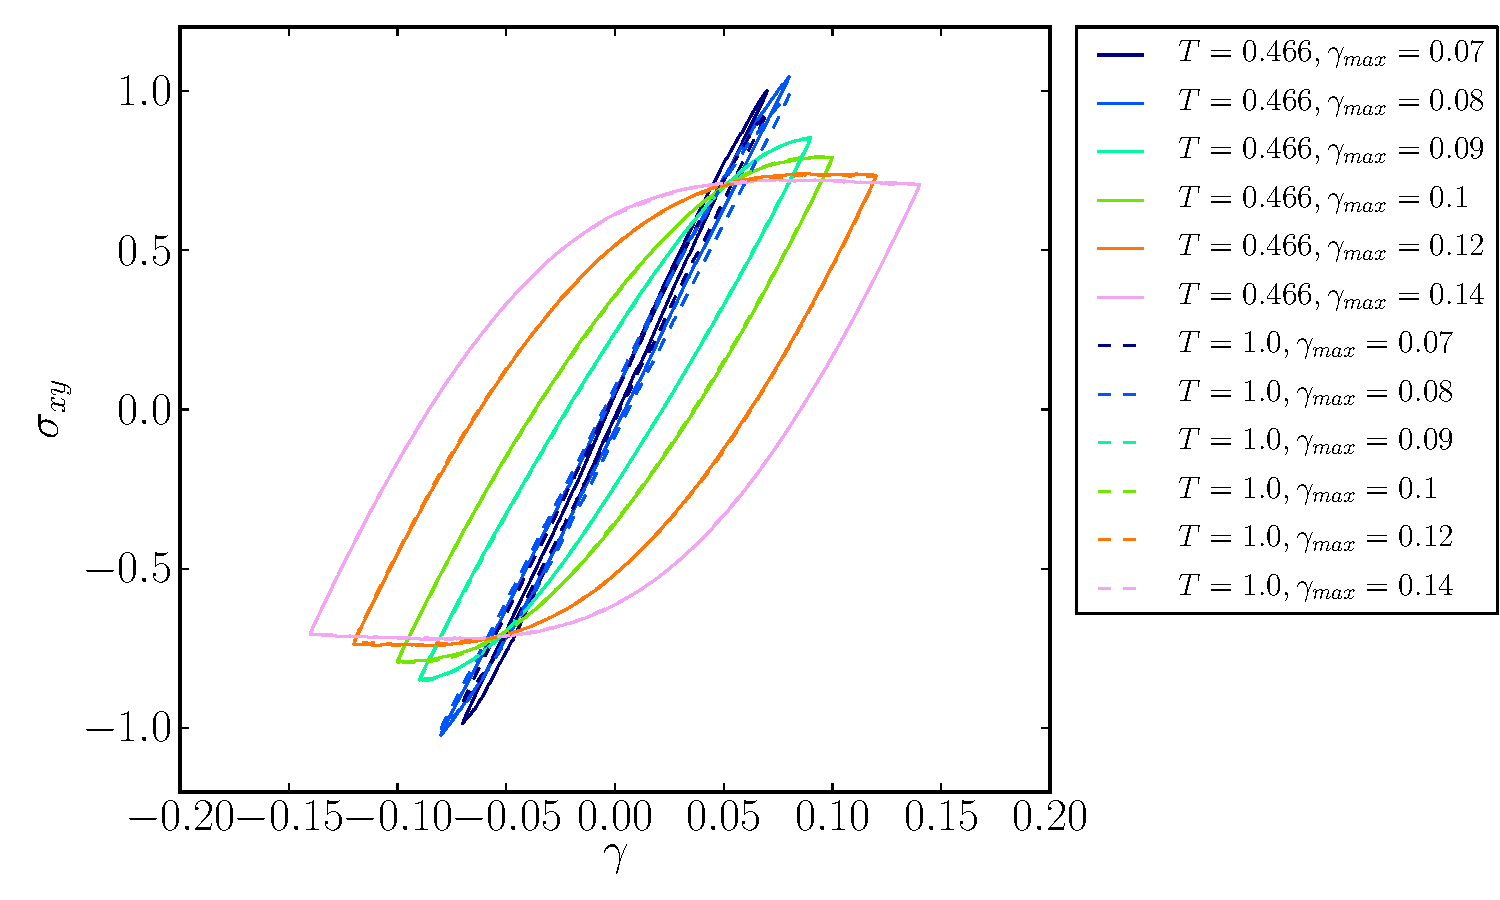
\includegraphics[width=0.8\textwidth]{HisteresisKA4000.pdf} 
\caption{Average stress in the plane of deformation as a function of shear strain, averaged on deformation cycles such that $\gamma_{acc} > \widetilde{\gamma}_{acc}$ on systems with $N=4000$. The systems show wide hysteresis for high $\gamma_{max}$, whereas at smaller $\gamma_{max}$ the curve almost retraces itself when strain is reversed. This indicated that dissipation is much higher at larger values of $\gamma_{max}$. \label{fig:Hysteresis}}
\end{figure}

It is meaningful to plot the values of the areas of the hysteresis curves in \autoref{fig:Hysteresis} as a function of $\gamma_{max}$. This is done in \autoref{fig:HysteresisAreas}, where the values are seen to increase dramatically after some threshold value of $\gamma_{max}$ which appears compatible with the $\gamma_{c}$ extracted from the fits of particle diffusion in \autoref{sec:DiffusionBehavior}. In other words, the onset of particle diffusion at $\gamma_{c}$ marks also the start of energy dissipation. \\
The exact dependence of the areas of the hysteresis curves as a function of $\gamma_{max}$ is not known to us. This stems from the fact that we didn't build a model for the dependence of $\sigma_{xy}$ as a function of the shear strain $\gamma$. However, for large values of $\gamma_{max}$ the hysteresis curve becomes just ``longer'' on the strain axis of the stress-strain curve, and thus its area is expected to be linear in $\gamma_{max}$.

\begin{figure}[!h] 
\centering 
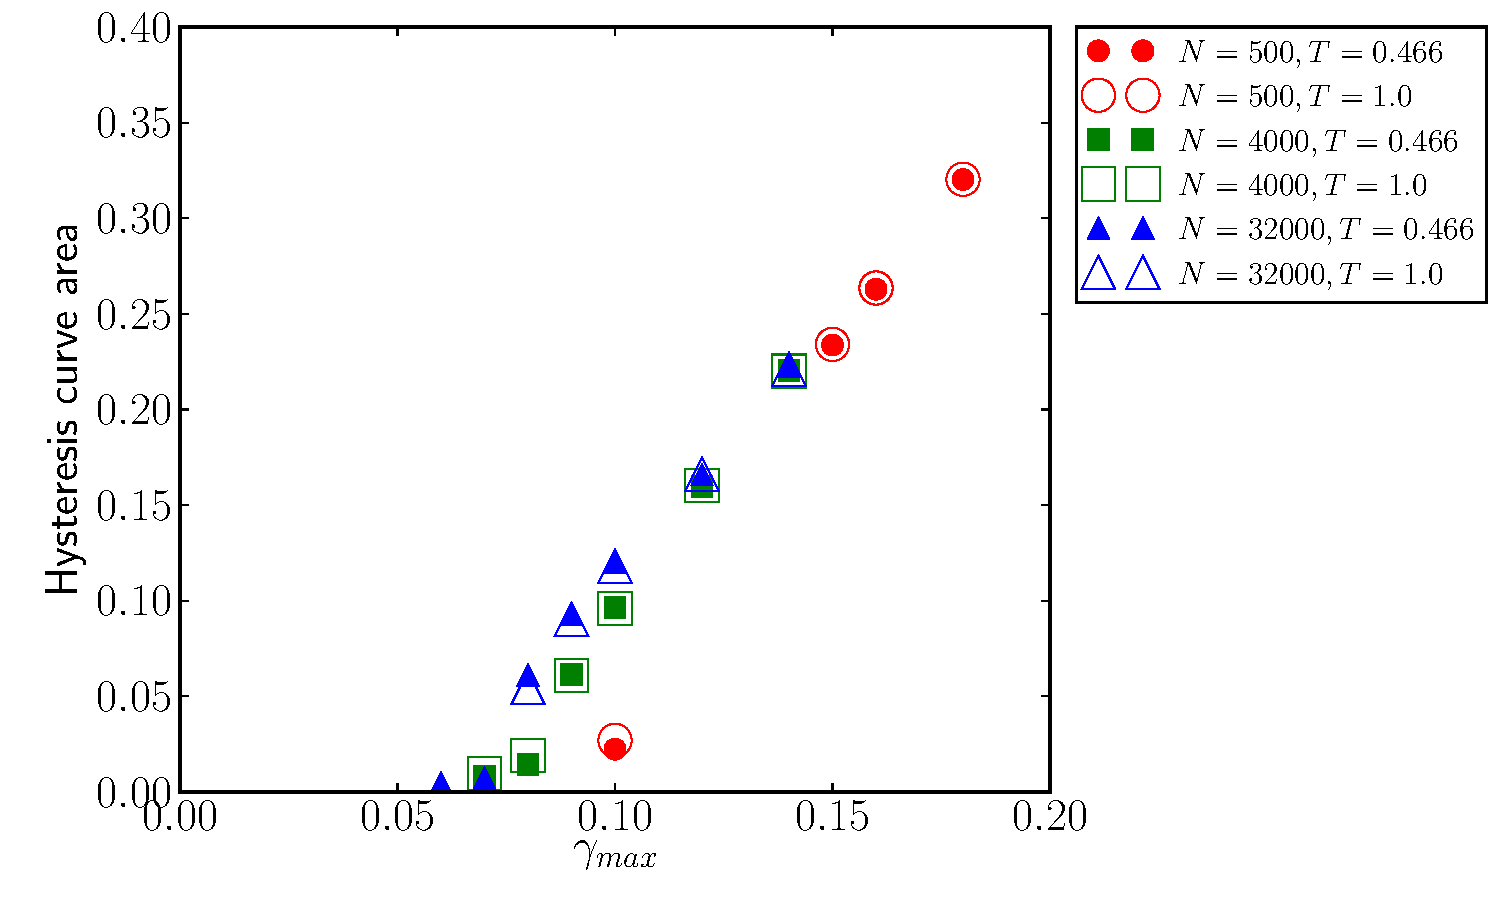
\includegraphics[width=0.8\textwidth]{Dissipation.pdf} 
\caption{Areas of hysteresis curves like those in \autoref{fig:Hysteresis} as a function of $\gamma_{max}$ for different system sizes. It's evident how dissipation sets in at a some value $\gamma_{max}$ that depends on the system size. Incidentally, this value is compatible with the values of $\gamma_{c}$ obtained from the analysis of the diffusion for the respective system size. As expected, for large values of $\gamma_{max}$ the hysteresis area approaches a linear behavior. \label{fig:HysteresisAreas}}
\end{figure}

\subsection{Is $\gamma_{c}$ equal to the yield strain?}

We've seen above that one can identify an amplitude $\gamma_{c}$ which is convincingly related to a slowdown in the relaxation of $U$ as a function of $\gamma_{acc}$ (\autoref{sec:EnergyBehavior}), the onset of particle diffusion (\autoref{sec:DiffusionBehavior}) and that of dissipation (\autoref{sec:DissipationBehavior}). Can the value of $\gamma_{c}$ be related to other relevant strain values? One possible candidate is the \emph{yield strain} $\gamma_{y}$, which we define here as the maximum of the stress-strain curve. To calculate $\gamma_{y}$ from our simulations, we take inherent structures at effective $T=0.466$ and subject them to shear deformation up to some large value of the strain. As seen above, the stress-strain curve is initially linear, but eventually saturates to a plateau value. Depending on the effective $T$ curves can peak in correspondence of some value that we identify as $\gamma_{y}$ (see \autoref{fig:YieldStrain}). Such value can be determined with precision by fitting a quadratic curve on the peak of the stress curve.\\
How does $\gamma_{y}$ compare to the values of $\gamma_{c}$ measured from systems with the same size and initial effective temperature? As it can be seen from \autoref{fig:YieldStrainVsCriticalStrain} the values do not seem to match.
At first sight, this could sound somewhat surprising: $\gamma_{c}$ is related to the onset of dissipation in the samples, which will set in as samples leave the elastic regime and exhibit a peak in the stress at $\gamma_{y}$. Strictly speaking, however, $\gamma_{y}$ is a property of initially \emph{undeformed} structures, because it is measured starting from samples that haven't experienced any prior deformation; $\gamma_{c}$, instead, is a property of oscillatory deformed samples that have undergone deformation and have consequently reached a ``steady'' state. Thus, there is no reason for $\gamma_{c}$ to coincide with $\gamma_{y}$, as they are associated to quite different objects.
In addition, we don't expect the discrepancy between $\gamma_{c}$ and $\gamma_{y}$ to be influenced by our choice of definition of $\gamma_{y}$. In fact, as stress-strain curves in \autoref{fig:YieldStrain} relative to different $N$ do almost overlap, any definition of $\gamma_{y}$ will give values of $\gamma_{y}$ that depend on $N$ very weakly, whereas $\gamma_{c}$ is significantly influenced by system size.

\begin{figure}[!h] 
\centering 
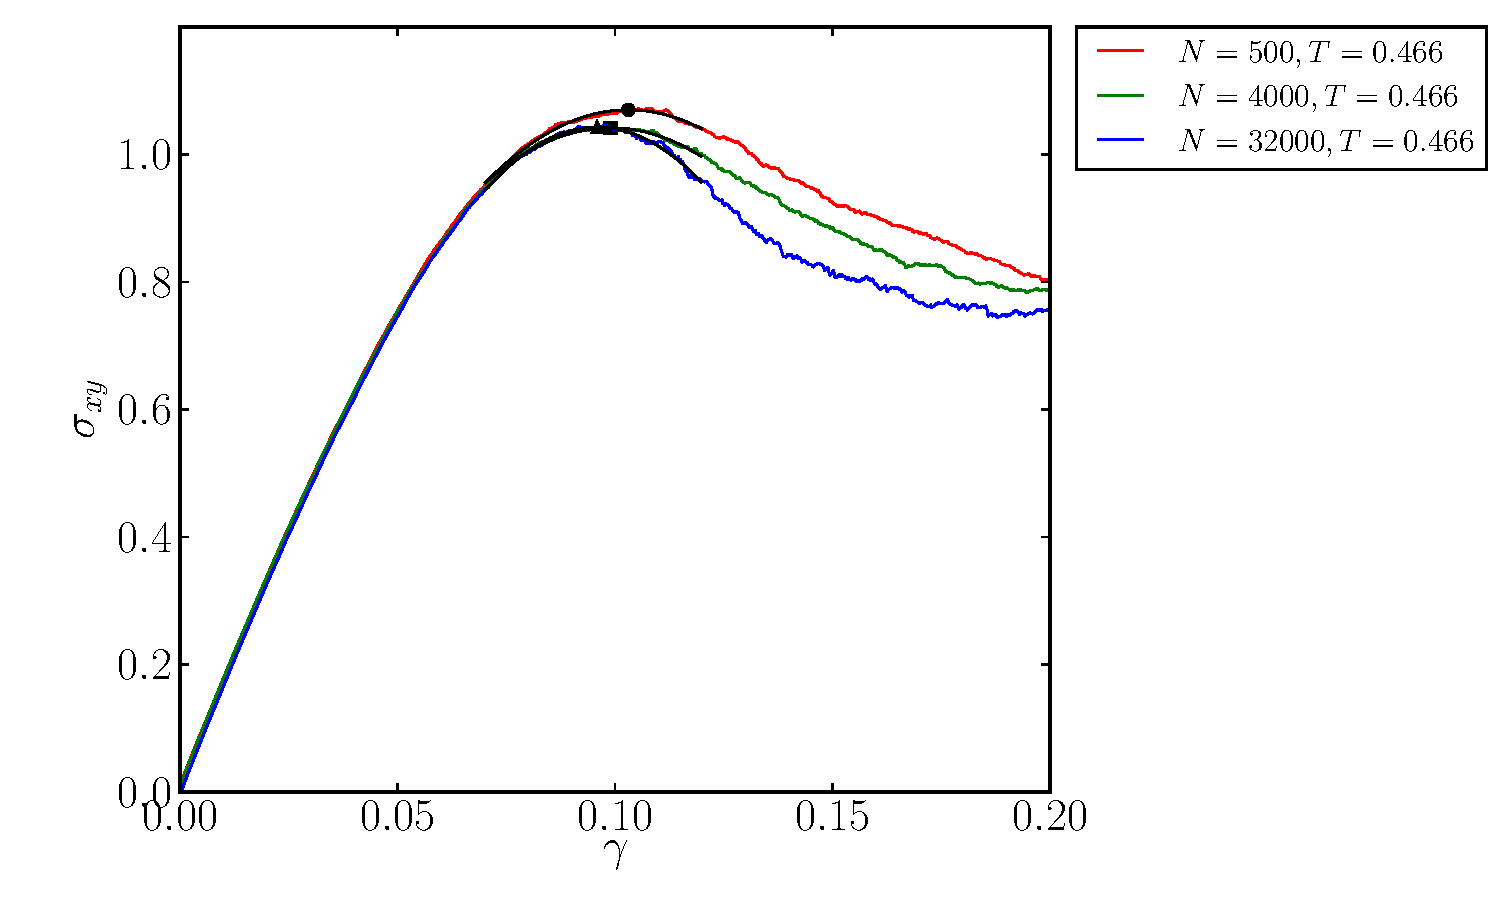
\includegraphics[width=0.8\textwidth]{Yield.pdf} 
\caption{Stress in the plane of deformation plotted as a function of strain starting from undeformed samples with $N=4000$. Stress at low $\gamma$ is linear, and then it peaks in correspondence of a value of the strain $\gamma_{y}$. The value of $\gamma_{y}$ is calculated by fitting the peak of the curve with a quadratic function. The value of $\gamma_{y}$ has a weak dependence on the size of the system. \label{fig:YieldStrain}}
\end{figure}

\begin{figure}[!h] 
\centering 
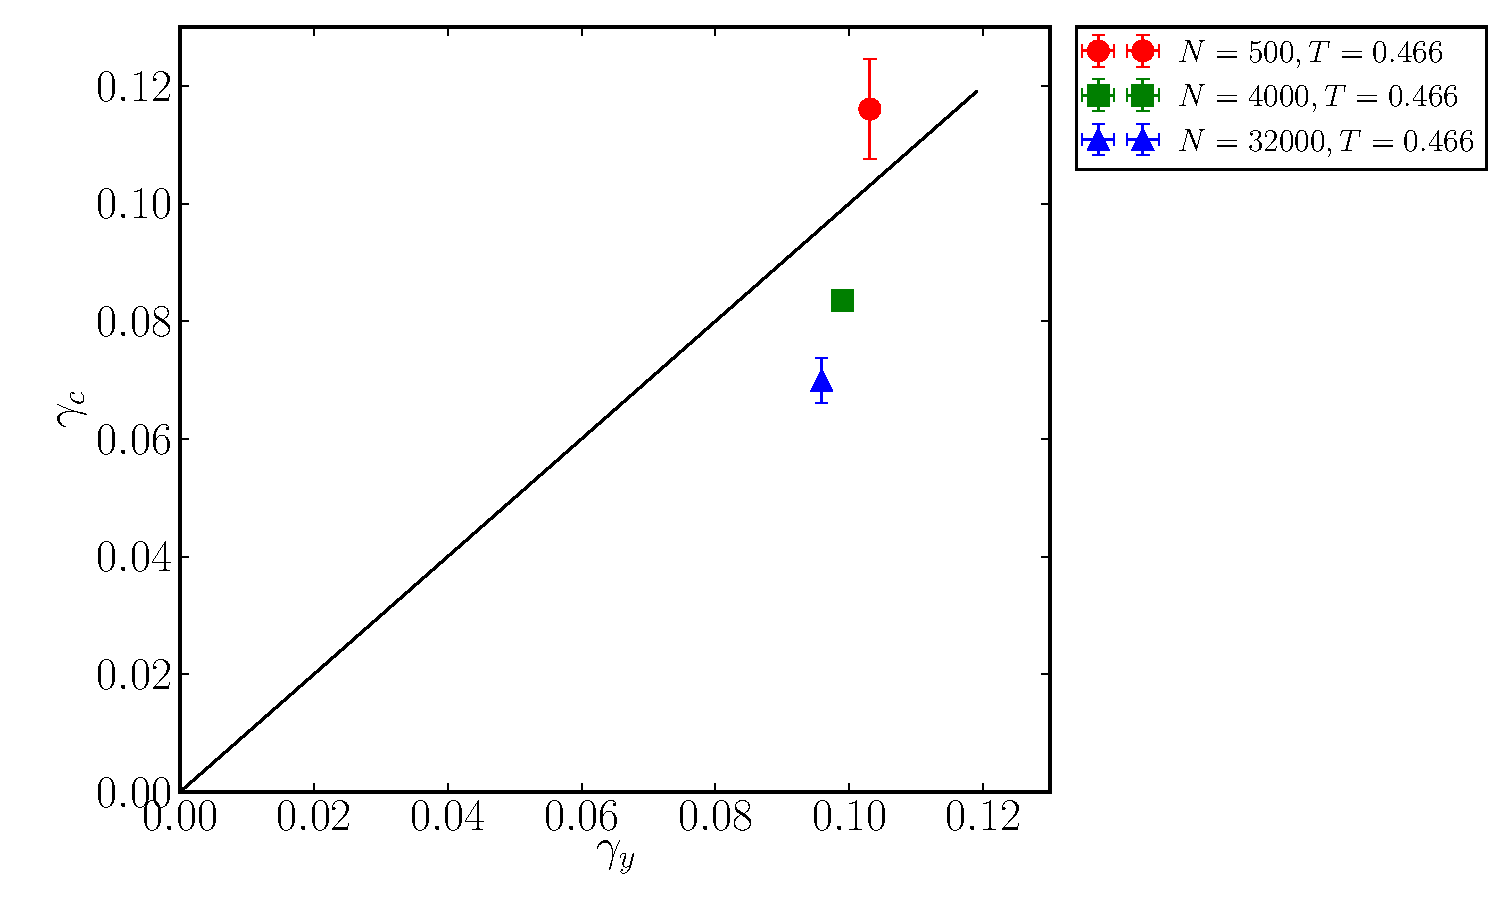
\includegraphics[width=0.8\textwidth]{YieldComparison.pdf} 
\caption{Values of $\gamma_{c}$ determined from the fits in \autoref{fig:DVsGammaMax} of the diffusion against the values of $\gamma_{y}$ determined from the fits in \autoref{fig:YieldStrain}. \label{fig:YieldStrainVsCriticalStrain}}
\end{figure}

\section{Summary}
We have performed simulations of oscillatory athermal shear deformation of dense binary mixtures of Lennard-Jones particles. \\
Our main finding is the existence of a ``critical'' shear deformation amplitude $\gamma_{c}$ which has a crucial role in the dynamics of our system under deformation. \\
Below $\gamma_{c}$, particle motion comes to a stop after a finite number of cycles, with samples reaching absorbing states that are invariant under the application of additional deformation cycles and are correlated with the starting configurations prior to deformation. Consequently, upon deformation, the average potential energy of the samples reaches a fixed value that depends on the initial effective $T$ and on the amplitude of the deformation $\gamma_{max}$ (\autoref{fig:UvsAccumulatedStrainKA}). The amount of cycles needed to reach such fixed value depends on the oscillation amplitude $\gamma_{max}$, and is seen to increase dramatically as $\gamma_{max}$ approaches $\gamma_{c}$ (\autoref{fig:CharacteristicRelaxationStrainVsAccumulatedStrain}). 
Absorbing states below $\gamma_{c}$ are characterized by narrow hysteresis curves and by a low amount of energy dissipation (\autoref{fig:Hysteresis} and \autoref{fig:HysteresisAreas}).\\
Above $\gamma_{c}$, systems move indefinitely in configuration space as more and more deformation cycles are performed. Motion under cyclic deformation is characterized by loss of memory of the initial effective temperature $T$. In fact, after some number of deformation cycles, samples assume states whose potential energy fluctuates around a value that depends on $\gamma_{max}$ only. The number of cycles needed to reach such steady energy state depends on $\gamma_{max}$, and increses as $\gamma_{max}$ approaches $\gamma_{c}$. In this regime samples exhibit large values of energy dissipation per cycle, and wide hysteresis curves. \\
By looking at the mean squared displacement of samples with $\gamma = 0$, the overall particle dynamics both below and above $\gamma_{c}$ can be approximated as a random walk of walkers having a finite probability to halt their motion (\autoref{fig:MSD0VsAccumulatedStrain}). In the steady state, a simple linear model is able to describe the MSD of the systems (\autoref{fig:MSDVsAccumulatedStrain}). Interestingly, the diffusion constants measured for the various systems can be described by a power-law model (\autoref{eq:DPowerLaw}). This is the same model used to fit the behavior of noncolloidal suspensions in \cite{corte2008random} (see \autoref{eq:ActiveFractionVsGammaMax}). The power-law behavior observed in noncolloidal suspensions was rationalized in \cite{corte2008random} by means of a mapping to the problem of conserved directed percolation \cite{menon2009universality}, which exhibits a non-equilibrium transition. However, it is not clear how a dense system like ours could be mapped onto a directed percolation problem \cite{ramaswamy2012private}. In this sense, more precise measurements of the characteristic accumulated strain needed to reach asymptotic values of the potential energy under deformation and more precise data about particle diffusion in the vicinity of $\gamma_{c}$ could allow to place our systems into a non-equilibrium universality class. \\
The analysis of particle motion under deformation reveals another interesting detail: for our largest system size ($N=32000$) we observe that above $\gamma_{c}$ particles that move the most organize in bands (\autoref{fig:ShearBands}) that occupy the same position in the simulation box as more and more deformation cycles are performed. To our knowledge, this is the first observation of ``shear bands'' in simulations of systems under oscillatory shear employing Lees-Edwards boundary conditions. The spatial heterogeneity in particle motion suggests that particle diffusion won't be isotropic (for instance, particles in a band will preferentially move in the plane of the band rather than orthogonally to it), and can't thus be described by simple isotropic diffusion. A more detailed analysis of such features of the dynamics would allow to explore all these aspects quantitatively. \\
The value of $\gamma_{c}$ has been compared to that of yield strain $\gamma_{y}$. Several definitions of $\gamma_{y}$ exists, and in our case we have considered $\gamma_{y}$ to be the strain corresponding to the peak in the shear stress-strain curve (\autoref{fig:YieldStrain}). Even though the two values must be correlated (in fact, there can't be particle diffusion without the system deviating from a perfectly elastic behavior and thus ``yielding'' in some way), they refer to the properties of quite different objects: $\gamma_{c}$ is extrapolated from the properties of oscillatory deformed samples in their steady state, whereas $\gamma_{y}$ is a property of undeformed samples. We indeed find that in our samples $\gamma_{c}$ and $\gamma_{y}$ are significantly different at the different system sizes that we have analyzed (\autoref{fig:YieldStrainVsCriticalStrain}). In addition, we don't expect this result to be influenced by our choice of definition of $\gamma_{y}$.\\
Even though the value of $\gamma_{c}$ shows a significant size dependence, our data in \autoref{fig:CriticalGammaVsInverseSize} suggest that $\gamma_{c}$ will remain larger than 0 as $N$ becomes large. This makes us conclude that our results (and in particular the existence of a transition at $\gamma_{c}$), even though affected by finite size effects, will be valid at macroscopic scales.

